%%%%%%%%%%%%%%%%%%%%%%%%%%%%%%%		CHAP 1		%%%%%%%%%%%%%%%%%%%%%%%%%%%%%%%

\clearpage
\chapter{Neutrinos in the Standard Model}
\label{cha:intro}

The Standard Model (SM) is a renormalisable Yang-Mills theory~\cite{Yang:1954ek} that describes the strong, %
electromagnetic, and weak interactions of elementary particles in the framework of quantum field %
theory~\cite{Glashow:1961tr, Weinberg:1967tq, Salam:1968rm}.
It is based on the local gauge symmetry group 
\begin{equation}
	\label{eq:smgroup}
	\text{SU(3)}_C \otimes \text{SU(2)}_L \otimes \text{U(1)}_Y
\end{equation}
where $C$, $L$ and $Y$ denote respectively colour, left-handed chirality and weak hyper-charge.
The gauge group uniquely determines the interactions and the number of %
vector gauge bosons that correspond to the generators of the group.
%
The electroweak subgroup $\text{SU(2)}_L \otimes \text{U(1)}_Y$ undergoes a spontaneous symmetry breaking process %
out of which three of the four vector bosons acquire mass ($W^\pm$ and $Z$~bosons) and the last one, the photon, remains massless.
This process requires at least one scalar boson with a non-zero vacuum expectation value~\cite{Higgs:1964pj, Higgs:1964ia}.
The colour symmetry does not break and does not mix with the electroweak sector. 
The generators of its algebra correspond to eight massless gluons.
The gauge and scalar bosons are coupled to fermion fields, which are irreducible representation of %
the Poincaré group.
The known elementary fermions are divided in two categories: quarks and leptons.
They are distinguished by the fact that quarks participate in all the interactions % 
whereas leptons participate only in the electroweak interactions.
%%In the SM, electroweak interactions can be studied separately from strong interactions, %
%%because the symmetry under the color group is unbroken and there is no mixing %
%%between the SU(3)$_C$ and the $\mathrm{SU(2)}_L \otimes \mathrm{U(1)}_Y$ sectors.
%%On the other hand, the Glashow, Salam, and Weinberg theory well explains the group mixing between %
%%electromagnetic and weak interactions caused by a symmetry breaking process.
%%They are eight massless gluons that mediate strong interactions, %
%%corresponding to the eight generators of SU(3)$_C$, and four gauge bosons, %
%%of which three are massive ($W^\pm$ and $Z$) and one is massless, corresponding %
%%to the three generators of SU(2)$_L$ and one generator of U(1)$_Y$, responsible for %
%%electroweak interactions.
Since the number and properties of the gauge bosons are determined by the SM group, %
the only independent parameters left are the coupling constants of the interactions, which can be determined by experiments.
%The spontaneous breaking symmetry requires at least one scalar boson thanks to the Higgs mechanism.
%The recent discovery of the Higgs boson is the crowning achievement of the SM~\ref{}.
%The symmetry group of the SM fixes the interactions, i.e. the number and properties of the %
%vector gauge bosons, with only three independent unknown parameters: the three coupling constants of %
%the SU(3)$_C$, SU(2)$_L$, and U(1)$_Y$ groups, all of which must be determined from experiments.
The number and the masses of scalar bosons and fermions are also to be determined experimentally, %
keeping in mind that they must transform according to the representations of the symmetry group %
and the fermion representations must lead to the cancellation of quantum anomalies.

\iffalse
\begin{center}
	\small
	\begin{tabular}{lccc}
		\toprule
		\textbf{Generation}	&\textbf{1st}	& \textbf{2nd}	& \textbf{3rd}	\\
		\midrule
		\multirow{2}*{Quark} & $u$ 		& $c$		& $t$		\\
		& $d$		& $s$		& $b$		\\
		\midrule
		\multirow{2}*{Leptons}	& $e$ 		& $\mu$		& $\tau$	\\
		& $\nu_e$	& $\nu_\mu$	& $\nu_\tau$	\\
		\bottomrule
	\end{tabular}
\end{center}
\fi

%In the SM, electroweak interactions can be studied separately from strong interactions, %
%because the symmetry under the color group is unbroken and there is no mixing %
%between the SU(3)$_C$ and the $\mathrm{SU(2)}_L \otimes \mathrm{U(1)}_Y$ sectors.
%On the other hand, the Glashow, Salam, and Weinberg theory well explains the group mixing between %
%electromagnetic and weak interactions caused by a symmetry breaking process.
%This model and the discovery of the predicted $W$ and $Z$ bosons, in addition to the gluon, %
%the top, and charm quarks, made the fortune of the Standard Model.
%Their redicted properties were experimentally confirmed with good precision and %
%the recent discovery of the Higgs Boson is the last crowning achievement of SM.

Despite being the most successful theory of particle physics to date, the SM is actually limited %
in its description of reality, in that some evidence is not explained nor addressed.
The most outstanding breakthrough is the discovery of neutrino oscillation, which was awarded the Nobel Prize in Physics in 2015 %
and has proven that the neutrinos are not all massless, as was assumed by the theory.	%% ??
Mass terms for the neutrinos can be included in the SM, with the implications of theoretical and naturalness problems.
Likewise, the SM is unable to provide an explanation of the observed asymmetry between matter and antimatter.
It was noted by Sakharov that a solution to this puzzle would require some form of C and CP violation %
in the early Universe, along with Baryon number violation and out-of-equilibrium interactions~\cite{Sakharov:1967dj}.
There is also plenty of evidence suggesting the presence of dark matter %
in the Universe~\cite{Zwicky:1933gu, Rubin:1970zza, Aghanim:2018eyx}, %
and there are a variety of theoretical and experimental endeavours trying to unearth its nature.
These facts suggest that the Standard Model is not a complete theory and additional physics %
Beyond the Standard Model (BSM) is required.

The study of neutrinos is for sure one of the most promising probes to BSM physics and %
is of vital importance to the future development of particle physics, %
in particular through precision measurement of their interactions.
A deep understanding of neutrino interactions, and neutrino-nucleon interactions in particular, %
could lead to a great impact on long-baseline experiments, proton decay searches, and supernova detection.
Since the SM is a renormalisable theory, even its quantum corrections are insensitive to the physics beyond the SM.
For this reason, the SM is phenomenologically very successful and so far has been able to describe all the known
phenomena, except for the indications in favour of neutrino oscillations, as it will be discussed in the following chapters.

\section{Electroweak sector}
\label{sec:ew_sector}

The electroweak (EW) sector of the SM is formed by the direct product of the weak isospin group $\text{SU(2)}_L$ and %
the hyper-charge group $\text{U(1)}_Y$.
The two groups are connected by the Gell-Mann--Nishijima~\cite{Nakano:1953zz, Gell-Mann:1956iqa} %
relation which connects the $I_3$ component of the weak isospin operator and the hyper-charge operator $Y$ %
with the charge operator $Q$ as
\begin{equation}
	\label{eq:gellmann}
	Q = I_3 + \frac{Y}{2}\ .
\end{equation}
Left-handed chiral components of the fermion fields form doublets under $\text{SU(2)}_L$
\begin{equation}
	\label{eq:doublets}
	\bs{L}_L = \mqty(\bs{\nu}_L \\ \bs{\ell}_L) \quad, \quad
	\bs{Q}_L = \mqty(\bs{q}_L^U \\ \bs{q}_L^D) \ ,
\end{equation}
where the left-handed fields (in bold-face) represent the fermion families
\begin{equation}
	\bs{\nu}_L  = \mqty(\nu_{eL} \\ \nu_{\mu L} \\ \nu_{\tau L}) \quad , \quad
	\bs{\ell}_L = \mqty(e_L \\ \mu_L \\ \tau_L) \quad , \quad
	\bs{q}^D_L  = \mqty(d_L \\ s_L \\ b_L) \quad , \quad \text{and} \quad
	\bs{q}^U_L  = \mqty(u_L \\ c_L \\ t_L)\ .
\end{equation}
%$\bs{q}^U$ and $\bs{q}^D$ represent respectively the up quark and down quark families.
The right-handed fields, instead, transform simply as singlets and they are
\begin{equation}
	\bs{\ell}_R = \mqty(e_R \\ \mu_R \\ \tau_R) \quad , \quad
	\bs{q}^D_R  = \mqty(d_R \\ s_R \\ b_R) \quad , \quad \text{and} \quad
	\bs{q}^U_R  = \mqty(u_R \\ c_R \\ t_R)\ .
\end{equation}
The right-handed components of the neutrino fields, $\nu_{\alpha R}$, are not historically considered in the SM %
because the neutrinos are assumed to be massless and the $\nu_R$ components are \emph{sterile} under any charge of the SM.
Furthermore, the helicity of neutrinos was measured to be consistent with left chirality~\cite{Goldhaber:1958nb}.
The EW Lagrangian is therefore the most general renormalisable Lagrangian invariant %
under the local symmetry $\text{SU(2)}_L \otimes \text{U(1)}_Y$:
\begin{align}
	\label{eq:ew_lagrangian}
	\mathcal{L}_\text{EW} =\  &i\, \cj{\bs{L}}_L\, \sh{D}\, \bs{L}_L + i\, \cj{\bs{Q}}_L\, \sh{D}\, \bs{Q}_L + %
			 i\, \cj{\bs{\ell}}_R\, \sh{D}\, \bs{\ell}_R + i\, \cj{\bs{q}}^D_R\, \sh{D}\, \bs{q}^D_R + %
			 i\, \cj{\bs{q}}^U_R\, \sh{D}\, \bs{q}^U_R \notag \\ 
			&-\frac{1}{4} B_{\mu\nu} B^{\mu\nu} - \frac{1}{4} \vb{A}_{\mu\nu} \vb{A}^{\mu\nu} 
		      + (D_\mu H)^\dagger (D^\mu H) - \mu^2 H^\dagger H - \lambda (H^\dagger H)^2  \notag \\
		      &- \qty( \cj{\bs{L}}_L\, Y^\ell H \,\bs{\ell}_R 
		      	     + \cj{\bs{Q}}_L\, Y^D    H \,\bs{q}^D_R 
		      	     + \cj{\bs{Q}}_L\, Y^U    \widetilde{H}\, \bs{q}^U_R \ +\ \text{h.c.})\ ,
\end{align}
where the covariant derivative is defined as 
\begin{equation}
	\label{eq:covariant}
	D_\mu = \pd_\mu + i g\, \vb{A}_\mu \cdot \vb{I} + i g'\, B_\mu \frac{Y}{2}\ ,
\end{equation}
and satisfies gauge invariance, %
and $\widetilde{H} = i \sigma_2 H^*$ is the conjugate Higgs field. % thanks to the transformations
It is important to note that Dirac mass terms for fermion fields other than neutrinos %
are anyway forbidden by the gauge symmetry.
These terms will become manifest once the symmetry is broken through the Higgs mechanism (see \refsec{sec:ew_higgs}).
%\begin{align}
%	\label{eq:gauge}
%	\vb{A}_\mu \cdot \vb{I} \longmapsto 
%\end{align}
The vector boson fields $\vb{A}^\mu = (A_1^\mu, A_2^\mu, A_3^\mu)$ and $B^\mu$ correspond respectively %
to the three generators $\vb{I} = (I_1, I_2, I_3)$ of the $\text{SU(2)}_L$ group %
and the generator $Y$ of the $\text{U(1)}_Y$ group.
The $\text{SU(2)}_L$ generators are $I_a = \sigma_a / 2$, with $\sigma_a$ the Pauli matrices, %
and thus satisfy the commutation relation
\begin{equation}
	\label{eq:generators}
	[I_a, I_b] = i\, \varepsilon_{a b c}\, I_c\ ,
\end{equation}
with $\varepsilon_{a b c}$ the Levi-Civita tensor.

\subsection{Electroweak interactions}
\label{sec:ew_interactions}

Expanding the covariant derivative and ignoring the kinetic terms, the interaction term for the leptonic sector is retrieved
\begin{equation}
	\label{eq:interaction}
	\mathcal{L}_\text{int,L} = -\frac{1}{2} \sum_\alpha %
		\mqty(\cj{\nu}_{\alpha L} & \cj{\ell}_{\alpha L}) %
		\mqty( g \sh{A}_3 - g' \sh{B} & g(\sh{A}_1 - i \sh{A}_2) \\
		       g(\sh{A}_1 + i \sh{A}_2) & - g \sh{A}_3 - g' \sh{B}  ) %
		\mqty(\nu_{\alpha L} \\ \ell_{\alpha L} ) - g'\, \cj{\ell}_{\alpha R}\, \sh{B} \, \ell_{\alpha R}\ ,
\end{equation}
where $\alpha$ is a family generation index.
Defining the combinations
\begin{align}
	\label{eq:fields}
	W^\mu &= \flatfrac{\qty(A_1^\mu - i A_2^\mu)}{\sqrt{2}} \\
	Z^\mu &= \cos \vartheta_\text{W} A_3^\mu - \sin \vartheta_\text{W} B^\mu \\
	A^\mu &= \sin \vartheta_\text{W} A_3^\mu + \cos \vartheta_\text{W} B^\mu \ ,
\end{align}
the electromagnetic field $A^\mu$ is expressed as a rotation of $A_3^\mu$ and $B^\mu$, thus recovering QED; %
the new field $Z^\mu$ also describes a neutral current process.
The Lagrangian in \refeq{eq:interaction} can therefore be divided into two parts, %
$\mathcal{L}_\text{int,L} = \mathcal{L}_\text{CC,L} + \mathcal{L}_\text{NC,L}$, %
describing charged-current (CC) and neutral-current (NC) interactions.
These are
\begin{align}
	\label{eq:lagrangian_cc}
	\mathcal{L}_\text{CC,L} &= -\frac{g}{2\sqrt{2}}\ j^\mu_\text{CC,L} W_\mu + \text{h.c.} \ , \\
	\label{eq:lagrangian_nc}
	\mathcal{L}_\text{NC,L} &= -\frac{g}{2\cos\vartheta_\text{W}}\ j^\mu_\text{NC,L} Z_\mu
		     + g\sin\vartheta_\text{W}\  \cj{\bs{\ell}}\, \sh{A}\, \bs{\ell} \ ,
\end{align}
where the $W$ and $Z$ vector bosons have been factorised out, leaving the fermionic currents
\begin{align}
	\label{eq:lepton_cc}
	j^\mu_\text{CC,L} &= \cj{\bs{\nu}}\, \gamma^\mu(1-\gamma^5)\, \bs{\ell}\ , \\
	\label{eq:lepton_nc}
	j^\mu_\text{NC,L} &= \cj{\bs{\nu}}\, \gamma^\mu\, (g^\nu_V - g^\nu_A \gamma^5)\, \bs{\nu} + %
		      \cj{\bs{\ell}}\, \gamma^\mu\, (g^\ell_V-g^\ell_A\gamma^5)\, \bs{\ell}\ .
\end{align}
The constant $g'$ has been re-written in terms of $g$ and $\vartheta_\text{W}$ by setting to zero the coupling of neutrinos %
to the electromagnetic field for neutrinos, which gives
\begin{equation}
	g\, \sin \vartheta_\text{W} = g'\, \cos \vartheta_\text{W}\ .
\end{equation}
The angle $\vartheta_\text{W}$ is known as Weinberg angle and it is estimated %
to be $\sin^2\vartheta_\text{W} \simeq 0.231$ from either neutrino neutral-current processes at low energies %
or the Z mixing with the photon in Drell-Yan processes at higher energies~\cite{Tanabashi:2018oca}.
Another important relation comes from the charged lepton couplings with the electromagnetic field which must coincide %
with the QED Lagrangian.
It follows that $g \sin\vartheta_\text{W} = q_e$ and so $g^2 + g'^2 = q_e^2$.
The~constants $g_V$ and $g_A$, introduced in \refeq{eq:lepton_nc}, can be defined for any fermion $\ferm$ as
\begin{equation}
	\label{eq:gv_ga}
	g_V^\ferm = I_3^\ferm - 2 q^\ferm \sin^2 \vartheta_\text{W} \quad \text{and} \quad
	g_A^\ferm = I_3^\ferm\ .
\end{equation}
Thanks to this notation, the interaction Lagrangians for the quark sector can be written in the same form of %
\refeqs{eq:lagrangian_cc}{eq:lagrangian_cc}, where the fermionic currents of \refeqs{eq:lepton_cc}{eq:lepton_nc} now become
\begin{align}
	\label{eq:quark_cc}
	j^\mu_\text{CC,Q} &= \cj{\bs{q}}^U\, \gamma^\mu(1-\gamma^5)\, \bs{q}^D\ , \\
	\label{eq:quark_nc}
	j^\mu_\text{NC,Q} &= \cj{\bs{q}}^U\, \gamma^\mu\, (g^U_V - g^U_A \gamma^5)\, \bs{q}^U + %
		      \cj{\bs{q}}^D\, \gamma^\mu\, (g^D_V-g^D_A\gamma^5)\, \bs{q}^D\ .
\end{align}

\subsection{Higgs mechanism}
\label{sec:ew_higgs}

In the EW Lagrangian in \refeq{eq:ew_lagrangian}, the Higgs $H$ is a complex scalar field and an $\text{SU(2)}_L$ doublet %
\begin{equation}
	\label{eq:higgs}
	H(x) = \mqty( H^+(x) \\ H^0(x) ) \ ,
\end{equation}
the potential of which can spontaneously break if $\lambda > 0$ and $\mu^2 < 0$, in
\begin{equation}
	\label{eq:higgs_potential}
	V(H) = \mu^2 H^\dagger H + \lambda (H^\dagger H)^2 \ .
\end{equation}
Defining
\begin{equation}
	\label{eq:vev}
	v \equiv \sqrt{- \frac{\mu^2}{\lambda}}\ ,
\end{equation}
the potential $V(H)$ shows a minimum for $H^\dagger H = v^2 / 2$, which %
corresponds to the lowest energy state, or vacuum.
In general, fermion and non-zero spin boson fields must have a vanishing vacuum expectation value (vev), %
so as to preserve the Lorentz symmetries of space and time.
The same applies to charged scalar fields, as the vacuum is electrically chargeless.
On the other hand, neutral scalar fields can have a nonzero value in vacuum, and so the vev %
of the Higgs field could be given by
\begin{equation}
	\expval{H} = \frac{1}{\sqrt{2}} \mqty( 0 \\ v )\ .
\end{equation}
This value spontaneously breaks the EW group $\text{SU(2)}_L \otimes \text{U(1)}_Y$, %
but it remains invariant under the gauge transformations from the $\text{U(1)}_Q$ group, %
with $Q$ from \refeq{eq:gellmann}, which guarantees the existence of a massless gauge boson %
associated with the photon.
Let us expand the scalar field around its vev and by choosing the unitary gauge three of the four real scalar fields %
can be rotated away being unphysical, simplifying to
\begin{equation}
	\label{eq:vev_higgs}
	H (x) = \frac{1}{\sqrt{2}} \mqty( 0 \\ v + h(x) )\ .
\end{equation}
Using the definition of the EW fields in \refeq{eq:fields}, %
the covariant derivative of \refeq{eq:covariant} applied to the Higgs field is 
\begin{equation}
	\label{eq:d_higgs}
	D_\mu H(x) = \frac{1}{\sqrt{2}} %
		\mqty ( i \frac{g}{\sqrt{2}} W_\mu (x) \qty[v + h(x)] \\ %
			\pd_\mu h(x) - i \frac{g}{2\cos \vartheta_\text{W}} Z_\mu(x) [v+h(x)] )\ .
\end{equation}
The Lagrangian terms with the Higgs field therefore becomes 
\begin{align}
	\label{eq:all_higgs}
	\mathcal{L}_\text{Higgs} =&\ \frac{1}{2} (\pd h)^2 - v^2 \lambda h^2 - \lambda h^3 - \frac{\lambda}{4} h^4 + %
			\frac{g^2 v^2}{4} W^\dagger_\mu W^\mu + \frac{g^2 v^2}{8\cos^2\vartheta_\text{W}} Z_\mu Z^\mu \notag \\
			& +\frac{g^2 v}{2} W^\dagger_\mu W^\mu h +\frac{g^2 v}{4\cos^2\vartheta_\text{W}} Z_\mu Z^\mu h \notag\\
			& +\frac{g^2}{4} W^\dagger_\mu W^\mu h^2 +  \frac{g^2}{8\cos^2\vartheta_\text{W}} Z_\mu Z^\mu h^2\ .
\end{align}
The second term of the first line is a mass term for the scalar field, %
from which the mass of the Higgs boson is determined to be $m_H = v \sqrt{2\lambda} = \sqrt{-2 \mu^2}$. %,
%a value recently measured~\ref{}.
The fifth and sixth terms represent the mass terms for the $W$ and $Z$ bosons, namely
\begin{equation}
	m_W = \frac{gv}{2} \quad, \quad m_Z = \frac{gv}{2\cos\vartheta_\text{W}}\ ,
\end{equation}
and the following parameter
\begin{equation}
	\label{eq:magic_ratio}
	\rho = \frac{m_W^2}{m_Z^2 \cos^2\vartheta_\text{W}}
\end{equation}
is predicted to be $\rho = 1$ in the SM. %: experimentally it is measured to be $\rho = 0.999999$.
The other terms of \ref{eq:all_higgs} describe self-interactions of the Higgs and %
interactions with the $W$ and $Z$ vector bosons.

Applying the same expansion of \refeq{eq:vev_higgs} to the Yukawa terms of the SM Lagrangian, %
couplings between left and right chiral fields and trilinear couplings of the fermions with the Higgs are obtained.
The lepton section becomes 
\begin{equation}
	\label{eq:lepton_mass}
	\mathcal{L}_{H, L} = - \frac{v}{\sqrt{2}}\ \cj{\bs{\ell}}_L\,Y^\ell\, \bs{\ell}_R %
			     - \frac{1}{\sqrt{2}}\ \cj{\bs{\ell}}_L\,Y^\ell\, \bs{\ell}_R\,h \ + \ \text{h.c.}\ ,
\end{equation}
and the same is found in the quark sector:
\begin{align}
	\mathcal{L}_{H, Q} = -& \qty(\frac{v}{\sqrt{2}}\ \cj{\bs{q}}_L^D Y^D \bs{q}_R^D %
			          + \frac{v}{\sqrt{2}}\ \cj{\bs{q}}_L^U Y^U \bs{q}_R^U) \notag\\ 
	\label{eq:quark_mass}
			     -& \qty(\frac{1}{\sqrt{2}}\ \cj{\bs{q}}_L^D Y^D \bs{q}_R^D\ h %
			          + \frac{1}{\sqrt{2}}\ \cj{\bs{q}}_L^U Y^U \bs{q}_R^U\ h) \,+\,\text{h.c.}
\end{align}

The terms in the Lagrangians of \refeqs{eq:lepton_mass}{eq:quark_mass} proportional to $\cj{\ferm}_L \ferm_R = \cj{\ferm}\, \ferm$ %
are Dirac mass terms for the fermion $\ferm$.
There is no principle by which the Yukawa coupling matrices $Y^\ferm$ should be diagonal \emph{a priori}, %
however without a diagonal matrix the fermion masses are not properly defined.
Being a generic complex matrix, the diagonalisation can be performed via a biunitary transformation
\begin{equation} 
	V^{\ferm\dagger}_L\ \qty(\frac{v}{\sqrt{2}} Y^\ferm)\ V^\ferm_R = \frac{v}{\sqrt{2}}\, \hat{Y}^\ferm_{\alpha} \equiv %
	\text{diag}\qty(\frac{y^\ferm_\alpha v}{\sqrt{2}})\ ,
\end{equation} 
where $V_L$ and $V_R$ are both unitary matrices.
The fermion masses are defined by the Yukawa couplings
\begin{equation}
	\label{eq:dirac_mass}
	m^\ferm_\alpha \equiv \frac{y^\ferm_\alpha v}{\sqrt{2}}\ ,
\end{equation}
with $\alpha$ a family generation index.
The biunitary transformation acts on the lepton fields as
\begin{equation}
	\label{eq:lepton_eigenmass}
	\hat{\bs{\ell}}_L = V^{\ell\dagger}_L\, \bs{\ell}_L \quad , \quad \hat{\bs{\ell}}_R = V^{\ell\dagger}_R\, \bs{\ell}_R
\end{equation}
and on the quark fields as 
\begin{align}
	\hat{\bs{q}}^D_L &= V^{D\dagger}_L\, \bs{q}^D_L \quad , \quad \hat{\bs{q}}^D_R = V^{D\dagger}_R\, \bs{q}^D_R \notag \\
	\label{eq:quark_eigenmass}
	\hat{\bs{q}}^U_L &= V^{U\dagger}_L\, \bs{q}^U_L \quad , \quad \hat{\bs{q}}^U_R = V^{U\dagger}_R\, \bs{q}^U_R\ ,
\end{align}
Dropping the ``hat notation'' to denote mass eigenfields, the lepton sector becomes
\begin{equation}
	\label{eq:lepton_diag}
	\mathcal{L}_\text{mass} = -\! \sum_{\alpha=e, \mu, \tau} \frac{y_\alpha^\ell v}{\sqrt{2}}\ \cj{\ell}_\alpha\, \ell_\alpha %
				= -\! \sum_{\alpha=e, \mu, \tau} m_\alpha\ \cj{\ell}_\alpha\, \ell_\alpha \ ,%
\end{equation}
and similarly the quark sector
\begin{align}
	\label{eq:quark_diag}
	\mathcal{L}_\text{mass} &= -\!\! \sum_{\alpha=d,s,b} \!\qty(\frac{y_\alpha^D v}{\sqrt{2}}\ \cj{q}^D_\alpha\, q^D_\alpha) %
				  -\!\! \sum_{\beta=u,c,t}  \!\qty(\frac{y_\alpha^U v}{\sqrt{2}}\ \cj{q}^U_\beta\,  q^U_\beta) \notag \\
				&= -\!\! \sum_{\alpha=d,s,b} \!\qty(m_\alpha\ \cj{q}^D_\alpha\, q^D_\alpha) %
				  -\!\! \sum_{\beta=u,c,t}  \!\qty(m_\beta \ \cj{q}^U_\beta\,  q^U_\beta)\ . %
\end{align}
As stressed previously, in the SM there are no right-handed neutrino fields, necessary for Dirac mass terms: %
the neutrinos are simply massless by definition.

\subsection{Fermion mixing}
\label{sec:fermion_mixing}

The same transformations of \refeqs{eq:lepton_eigenmass}{eq:quark_eigenmass} should be %
equally applied to all the parts of the EW Lagrangian.
Let us start from the quark charged current expressed in \refeq{eq:quark_cc}
\begin{equation}
	\label{eq:real_quark_cc}
	j^\mu_\text{CC,Q} = 2\ \cj{\bs{q}}^U_L\, \gamma^\mu\, \bs{q}^D_L %
			  = 2\ \cj{\hat{\bs{q}}}^U_L V^{U\dagger}_L\, \gamma^\mu\, V_L^D\hat{\bs{q}}^D_L % 
			  = 2\ \cj{\hat{\bs{q}}}^U_L\, \gamma^\mu\, V\, \hat{\bs{q}}^D_L\ ,
\end{equation}
where the unitary matrix $V = V^{U\dagger}_L V^D_L$, called Cabibbo-Kobayashi-Maskawa (CKM) matrix, %
describes the mixing between quark fields in weak interaction processes when initial and final states %
represent particles with definite masses.
The same mixing matrix however does not appear in the NC current of \refeq{eq:quark_nc}; %
defining the couplings $2\,g_L^\ferm = g_V^\ferm + g_A^\ferm$ and $2\,g_R^\ferm = g_V^\ferm - g_A^\ferm$, %
the current with mass eigenstates becomes
\begin{align}
	\label{eq:real_quark_nc}
	j^\mu_\text{NC,Q} &= 2\,g^U_L\ \cj{\bs{q}}^U_L\, \gamma^\mu\, \bs{q}^U_L %
			   + 2\,g^U_R\ \cj{\bs{q}}^U_R\, \gamma^\mu\, \bs{q}^U_R %
			   + 2\,g^D_L\ \cj{\bs{q}}^D_L\, \gamma^\mu\, \bs{q}^D_L %
			   + 2\,g^D_R\ \cj{\bs{q}}^D_R\, \gamma^\mu\, \bs{q}^D_R \notag \\
			  &= 2\,g^U_L\ \cj{\hat{\bs{q}}}^U_L V^{U\dagger}_L\, \gamma^\mu\, V^U_L \hat{\bs{q}}^U_L %
			   + 2\,g^U_R\ \cj{\hat{\bs{q}}}^U_R V^{U\dagger}_R\, \gamma^\mu\, V^U_R \hat{\bs{q}}^U_R \notag \\
			  &\hphantom{=} + 2\,g^D_L\ \cj{\hat{\bs{q}}}^D_L V^{D\dagger}_L\, \gamma^\mu\, V^D_L \hat{\bs{q}}^D_L %
			   + 2\,g^D_R\ \cj{\hat{\bs{q}}}^D_R V^{D\dagger}_R\, \gamma^\mu\, V^D_R \hat{\bs{q}}^D_R \notag \\
			  &= 2\,g^U_L\ \cj{\hat{\bs{q}}}^U_L \, \gamma^\mu\, \hat{\bs{q}}^U_L %
			   + 2\,g^U_R\ \cj{\hat{\bs{q}}}^U_R \, \gamma^\mu\, \hat{\bs{q}}^U_R %
			   + 2\,g^D_L\ \cj{\hat{\bs{q}}}^D_L \, \gamma^\mu\, \hat{\bs{q}}^D_L %
			   + 2\,g^D_R\ \cj{\hat{\bs{q}}}^D_R \, \gamma^\mu\, \hat{\bs{q}}^D_R \ .
\end{align}
The neutral current with massive fields has the same form of the neutral current with unrotated fields.
This is true also for the electromagnetic current of the EW Lagrangian.
This phenomenon is called Glashow-Iliopoulos-Maiani (GIM) mechanism~\cite{Glashow:1970gm}, by which %
flavour-changing neutral currents (FCNCs) are forbidden at tree level thanks to the unitarity of the weak interaction, %
but allowed in suppressed loop diagrams.

Looking at the lepton sector, the transformation of \refeq{eq:lepton_eigenmass} are not analogously defined for neutrino fields.
Therefore, neutrino states can be arbitrarily chosen such that $\hat{\bs{\nu}}_L = V^{\ell\dagger}_L\, \bs{\nu}_L$, %
where $V^\ell_L$ is the same of \refeq{eq:lepton_eigenmass}.
The lepton charged current becomes
\begin{equation}
	j^\mu_\text{CC,L} = 2\ \cj{\bs{\nu}}_L\, \gamma^\mu\, \bs{\ell}_L %
			  = 2\ \cj{\hat{\bs{\nu}}}_L V^{\ell\dagger}_L\, \gamma^\mu\, V^\ell_L\hat{\bs{\ell}}_L % 
			  = 2\ \cj{\hat{\bs{\nu}}}_L\, \gamma^\mu\, \bs{\hat{\ell}}_L\ .
\end{equation}
The fields $\hat{\bs{\nu}} = \qty(\hat{\nu}_e, \hat{\nu}_\mu, \hat{\nu}_\tau)$ are called \emph{flavour neutrino fields}, %
because they couple only to the corresponding charged lepton fields in the equation above.
As in the case of the quark fields, thanks to the unitarity of the matrices $V^\ell_L$ and $V^\ell_R$, %
the GIM mechanism applies even for the leptonic neutral current.





\section{Neutrino oscillations}
\label{sec:neutrino_oscillations}

As seen in \refsec{sec:ew_sector}, the SM does not consider right-handed neutrino fields.
For this reason, a Yukawa term coupling the lepton $\text{SU(2)}_L$ doublet with the conjugate Higgs field %
does not appear in the EW Lagrangian.
It follows that after the spontaneous symmetry breaking caused by the Higgs non-zero vev the neutrinos %
do not gain Dirac mass terms, as the other fermions do.
This ``asymmetry'' between fermion fields can be easily resolved by extending the SM and %
introducing the right-handed neutrino fields
\begin{equation}
	\bs{\nu}_R = \mqty(\nu_{eR} \\ \nu_{\mu R} \\ \nu_{\tau R})\ .
\end{equation}
Having now both chiralities, Dirac mass terms can be constructed for neutrinos, leading to neutrino mixing %
and so the neutrino oscillation phenomenon, observed in various neutrino experiments.

\subsection{Neutrino mixing}
\label{sec:neutrino_mixing}

Thanks to this extension, the following Yukawa term is now allowed
\begin{equation}
	\mathcal{L}_\text{EW} \supset - \qty( \cj{\bs{L}}_L\, Y^\ell H \,\bs{\ell}_R 
		      	     + \cj{\bs{L}}_L\, Y^\nu \widetilde{H}\, \bs{\nu}_R \ +\ \text{h.c.}) \ ,
\end{equation}
and using the expansion of \refeq{eq:vev_higgs} the Yukawa matrix can be diagonalised with a biunitary transformation %
to define masses for the neutrino fields.
This leads to new mass eigenfields
\begin{equation}
	\label{eq:neutrino_eigenmass}
	\hat{\bs{\nu}}_L = V^{\nu\dagger}_L\, \bs{\nu}_L = \mqty(\nu_{1L} \\ \nu_{2L} \\ \nu_{3L}) %
	\quad , \quad %
	\hat{\bs{\nu}}_R = V^{\nu\dagger}_R\, \bs{\nu}_R = \mqty(\nu_{1R} \\ \nu_{2R} \\ \nu_{3R})\ ,
\end{equation}
where the fields $\nu_i = \nu_{iL} + \nu_{iR}$ describe Dirac neutrinos with definite masses.
%Looking at the lepton sector, the transformation of \refeq{eq:neutrino_eigenmass} are not analogously defined for neutrino fields.
%Therefore, we can arbitrarily choose neutrino states such that $\hat{\bs{\nu}}_L = V^{\ell\dagger}_L\, \bs{\nu}_L \quad$, %
%where $V^\ell_L$ is the same of \refeq{eq:lepton_eigenmass}.
Having now neutrino mass eigenstates, the lepton charged current of \refeq{eq:lepton_cc} becomes
\begin{equation}
	j^\mu_\text{CC,L} = 2\ \cj{\bs{\nu}}_L\, \gamma^\mu\, \bs{\ell}_L %
			  = 2\ \cj{\hat{\bs{\nu}}}_L V^{\nu\dagger}_L\, \gamma^\mu\, V^\ell_L\hat{\bs{\ell}}_L % 
			  = 2\ \cj{\hat{\bs{\nu}}}_L\, \gamma^\mu\, U \bs{\hat{\ell}}_L\ ,
\end{equation}
where the unitary matrix $U = V^\nu_L V^\ell_L$ is completely analogous to the CKM matrix of the quark weak charged current.
This matrix is called Pontecorvo-Maki-Nakagawa-Sakata (PMNS) matrix.
Since the flavour of charged lepton is uniquely defined by their masses, it is customary to re-define %
the left-handed flavour neutrino fields as
\begin{equation}
	\bs{\nu}_L = U\, \hat{\bs{\nu}}_L\ ,
\end{equation}
which allows to write the charged current Lagrangian in terms of flavour neutrinos
being careful that, if neutrino masses are taken into account, mixing of the fields occurs:
\begin{align}
	\label{eq:lepton_cc_lagrangian}
	\mathcal{L}_\text{CC,L} &= -\frac{g}{\sqrt{2}} \sum_{\alpha=e,\mu,\tau} \cj{\nu}_\alpha\, \sh{W} (1-\gamma^5)\, \ell_\alpha %
					\ +\  \text{h.c.} \notag \\
				&= -\frac{g}{\sqrt{2}} \sum_{\alpha=e,\mu,\tau} \sum_{i=1}^3 U_{\alpha i}^*\, \cj{\nu}_i %
					\,\sh{W} (1-\gamma^5)\, \ell_\alpha \ + \ \text{h.c.}
\end{align}
The GIM mechanism is still valid and no mixing occurs in neutral current interactions.

\subsection{Propagation of neutrinos in vacuum}
\label{sec:neutrino_vacuum}

The effect of neutrino mixing is mostly visible in the propagation of neutrinos in space-time.
Neutrinos with flavour $\alpha$ are produced and detected in charged current interactions in association with %
a charged lepton, according to \refeq{eq:lepton_cc_lagrangian}.
Approximating the neutrino fields to plane-waves, the flavour states are described by
\begin{equation}
	\label{eq:neutrino_mix}
	\ket{\nu_\alpha} = \sum_i U^*_{\alpha i} \ket{\nu_i} \ ,
\end{equation}
where the mass eigenstates are orthonormal, $\braket{\nu_i}{\nu_j} = \delta_{ij}$, %
and thanks to the unitarity of the PMNS matrix the relation $\braket{\nu_\alpha}{\nu_\beta} = \delta_{\alpha \beta}$ holds.
It follows that the probability of producing and detecting a neutrino of the same flavour in the same point of space-time %
is, unsurprisingly, one.
However, in a typical neutrino experiment, production and detection of neutrinos happen in two different locations and times.
The massive neutrino states $\ket{\nu_i}$ are eigenstates of the Hamiltonian, with eigenvalues their energies:
\begin{equation}
	\label{eq:hamilton}
	\mathcal{H} \ket{\nu_i} = E_i \ket{\nu_i} = \sqrt{\vb{p}^2 + m_i^2} \ket{\nu_i}\ ,
\end{equation}
with $\vb{p}$ the momentum of the produced flavour neutrino.
The Hamiltonian dictates the time evolution of the states through the Schr{\"o}dinger's equation, and %
so assuming neutrinos evolve as plane waves a solution to the equation is given by
\begin{equation}
	\label{eq:neutrino_time}
	\ket{\nu_i(t)} = e^{-i E_i t} \ket{\nu_i}\quad \text{and} \quad %
	\ket{\nu_\alpha(t)} = \sum_i U^*_{\alpha i} e^{-i E_i t} \ket{\nu_i}\ .
\end{equation}
Using the relation of \refeq{eq:neutrino_mix}, the pure neutrino flavour state $\ket{\nu_\alpha(t)}$ at $t=0$ %
is expressed as a superposition of flavour states at time $t > 0$, as
\begin{equation}
	\label{eq:neutrino_time_flavour}
	\ket{\nu_\alpha(t)} = \sum_{\beta=e,\mu,\tau} \qty(\sum_i U^*_{\alpha i} e^{-i E_i t} U_{\beta i}) \ket{\nu_\beta}\ ,
\end{equation}
therefore the transition probability from a state $\nu_\alpha$ to a state $\nu_\beta$ over a certain amount of time $t$ is 
\begin{equation}
	\label{eq:oscillation_probability_bad}
	P(\nu_\alpha \to \nu_\beta) \equiv \qty|\braket{\nu_\alpha}{\nu_\beta(t)}|^2 = %
	\sum_{ij} U_{i\alpha}^* U_{\beta i} U_{\alpha j} U_{j\beta}^* %
	e^{-i(E_j - E_i)t}\ .
	%\exp \qty(-i \frac{\Delta m_{ij}^2 L}{2 E})\ ,
\end{equation}
For ultra relativistic neutrinos, the energies can be approximated by
\begin{equation}
	E_i \simeq E + \frac{m_i^2}{2E}\ ,
\end{equation}
and the propagation time is naturally replaced by the propagation length, i.e.\ $t \simeq L$, %
because it is easier to determine experimentally.
Adopting these approximations, the probability of \refeq{eq:oscillation_probability_bad} reads
\begin{equation}
	\label{eq:oscillation_probability}
	P(\nu_\alpha \to \nu_\beta) \equiv \qty|\braket{\nu_\alpha}{\nu_\beta(t)}|^2 = %
	\sum_{ij} U_{i\alpha}^* U_{\beta i} U_{\alpha j} U_{j\beta}^* %
	\exp \qty(-i \frac{\Delta m_{ij}^2 L}{2 E})\ ,
	%\exp \qty(-i \frac{\Delta m_{ij}^2 L}{2 E})\ ,
\end{equation}
where $\Delta m^2_{ij} = m_i^2 - m_j^2$ are the squared mass differences of the neutrinos.
The probability of \refeq{eq:oscillation_probability} is called \emph{oscillation probability} %
because it shows an oscillatory behaviour with respect to the ratio $\flatfrac{L}{E}$, %
while the other parameters---the PMNS matrix elements and the neutrino masses---are constant of nature.
The oscillation probability as a function of $\flatfrac{L}{E}$ is shown on \reffig{fig:osc_behave} %
for an initial $\nu_e$ and $\nu_\mu$.
The transition probability for $\alpha = \beta$ is usually called \emph{disappearance probability}, %
and for $\alpha \neq \beta$ is called \emph{appearance probability}, because experiments typically %
measure the amount of neutrinos of a certain flavour at the production site and at the detection site.

\begin{figure}
	\centering
	\resizebox{\linewidth}{!}{% GNUPLOT: LaTeX picture with Postscript
\begingroup
  \makeatletter
  \providecommand\color[2][]{%
    \GenericError{(gnuplot) \space\space\space\@spaces}{%
      Package color not loaded in conjunction with
      terminal option `colourtext'%
    }{See the gnuplot documentation for explanation.%
    }{Either use 'blacktext' in gnuplot or load the package
      color.sty in LaTeX.}%
    \renewcommand\color[2][]{}%
  }%
  \providecommand\includegraphics[2][]{%
    \GenericError{(gnuplot) \space\space\space\@spaces}{%
      Package graphicx or graphics not loaded%
    }{See the gnuplot documentation for explanation.%
    }{The gnuplot epslatex terminal needs graphicx.sty or graphics.sty.}%
    \renewcommand\includegraphics[2][]{}%
  }%
  \providecommand\rotatebox[2]{#2}%
  \@ifundefined{ifGPcolor}{%
    \newif\ifGPcolor
    \GPcolortrue
  }{}%
  \@ifundefined{ifGPblacktext}{%
    \newif\ifGPblacktext
    \GPblacktexttrue
  }{}%
  % define a \g@addto@macro without @ in the name:
  \let\gplgaddtomacro\g@addto@macro
  % define empty templates for all commands taking text:
  \gdef\gplbacktext{}%
  \gdef\gplfronttext{}%
  \makeatother
  \ifGPblacktext
    % no textcolor at all
    \def\colorrgb#1{}%
    \def\colorgray#1{}%
  \else
    % gray or color?
    \ifGPcolor
      \def\colorrgb#1{\color[rgb]{#1}}%
      \def\colorgray#1{\color[gray]{#1}}%
      \expandafter\def\csname LTw\endcsname{\color{white}}%
      \expandafter\def\csname LTb\endcsname{\color{black}}%
      \expandafter\def\csname LTa\endcsname{\color{black}}%
      \expandafter\def\csname LT0\endcsname{\color[rgb]{1,0,0}}%
      \expandafter\def\csname LT1\endcsname{\color[rgb]{0,1,0}}%
      \expandafter\def\csname LT2\endcsname{\color[rgb]{0,0,1}}%
      \expandafter\def\csname LT3\endcsname{\color[rgb]{1,0,1}}%
      \expandafter\def\csname LT4\endcsname{\color[rgb]{0,1,1}}%
      \expandafter\def\csname LT5\endcsname{\color[rgb]{1,1,0}}%
      \expandafter\def\csname LT6\endcsname{\color[rgb]{0,0,0}}%
      \expandafter\def\csname LT7\endcsname{\color[rgb]{1,0.3,0}}%
      \expandafter\def\csname LT8\endcsname{\color[rgb]{0.5,0.5,0.5}}%
    \else
      % gray
      \def\colorrgb#1{\color{black}}%
      \def\colorgray#1{\color[gray]{#1}}%
      \expandafter\def\csname LTw\endcsname{\color{white}}%
      \expandafter\def\csname LTb\endcsname{\color{black}}%
      \expandafter\def\csname LTa\endcsname{\color{black}}%
      \expandafter\def\csname LT0\endcsname{\color{black}}%
      \expandafter\def\csname LT1\endcsname{\color{black}}%
      \expandafter\def\csname LT2\endcsname{\color{black}}%
      \expandafter\def\csname LT3\endcsname{\color{black}}%
      \expandafter\def\csname LT4\endcsname{\color{black}}%
      \expandafter\def\csname LT5\endcsname{\color{black}}%
      \expandafter\def\csname LT6\endcsname{\color{black}}%
      \expandafter\def\csname LT7\endcsname{\color{black}}%
      \expandafter\def\csname LT8\endcsname{\color{black}}%
    \fi
  \fi
    \setlength{\unitlength}{0.0500bp}%
    \ifx\gptboxheight\undefined%
      \newlength{\gptboxheight}%
      \newlength{\gptboxwidth}%
      \newsavebox{\gptboxtext}%
    \fi%
    \setlength{\fboxrule}{0.5pt}%
    \setlength{\fboxsep}{1pt}%
\begin{picture}(14400.00,5760.00)%
    \gplgaddtomacro\gplbacktext{%
      \csname LTb\endcsname%%
      \put(618,595){\makebox(0,0)[r]{\strut{}0}}%
      \csname LTb\endcsname%%
      \put(618,1108){\makebox(0,0)[r]{\strut{}0.1}}%
      \csname LTb\endcsname%%
      \put(618,1620){\makebox(0,0)[r]{\strut{}0.2}}%
      \csname LTb\endcsname%%
      \put(618,2133){\makebox(0,0)[r]{\strut{}0.3}}%
      \csname LTb\endcsname%%
      \put(618,2646){\makebox(0,0)[r]{\strut{}0.4}}%
      \csname LTb\endcsname%%
      \put(618,3159){\makebox(0,0)[r]{\strut{}0.5}}%
      \csname LTb\endcsname%%
      \put(618,3671){\makebox(0,0)[r]{\strut{}0.6}}%
      \csname LTb\endcsname%%
      \put(618,4184){\makebox(0,0)[r]{\strut{}0.7}}%
      \csname LTb\endcsname%%
      \put(618,4697){\makebox(0,0)[r]{\strut{}0.8}}%
      \csname LTb\endcsname%%
      \put(618,5209){\makebox(0,0)[r]{\strut{}0.9}}%
      \csname LTb\endcsname%%
      \put(618,5722){\makebox(0,0)[r]{\strut{}1}}%
      \csname LTb\endcsname%%
      \put(720,409){\makebox(0,0){\strut{}\np{0.0}}}%
      \csname LTb\endcsname%%
      \put(1854,409){\makebox(0,0){\strut{}\np{0.5}}}%
      \csname LTb\endcsname%%
      \put(2988,409){\makebox(0,0){\strut{}\np{1.0}}}%
      \csname LTb\endcsname%%
      \put(4122,409){\makebox(0,0){\strut{}\np{1.5}}}%
      \csname LTb\endcsname%%
      \put(5255,409){\makebox(0,0){\strut{}\np{2.0}}}%
      \csname LTb\endcsname%%
      \put(6389,409){\makebox(0,0){\strut{}\np{2.5}}}%
    }%
    \gplgaddtomacro\gplfronttext{%
      \csname LTb\endcsname%%
      \put(126,3158){\rotatebox{-270}{\makebox(0,0){\strut{}Oscillation probability}}}%
      \csname LTb\endcsname%%
      \put(4121,130){\makebox(0,0){\strut{}Length / Energy / \np{e4} (km / GeV)}}%
      \csname LTb\endcsname%%
      \put(4237,5183){\makebox(0,0)[r]{\strut{}$\nu_e \to \nu_\tau$}}%
      \csname LTb\endcsname%%
      \put(4237,5369){\makebox(0,0)[r]{\strut{}$\nu_e \to \nu_\mu$}}%
      \csname LTb\endcsname%%
      \put(4237,5555){\makebox(0,0)[r]{\strut{}$\nu_e \to \nu_e$}}%
    }%
    \gplgaddtomacro\gplbacktext{%
      \csname LTb\endcsname%%
      \put(7421,595){\makebox(0,0)[r]{\strut{}}}%
      \csname LTb\endcsname%%
      \put(7421,1108){\makebox(0,0)[r]{\strut{}}}%
      \csname LTb\endcsname%%
      \put(7421,1620){\makebox(0,0)[r]{\strut{}}}%
      \csname LTb\endcsname%%
      \put(7421,2133){\makebox(0,0)[r]{\strut{}}}%
      \csname LTb\endcsname%%
      \put(7421,2646){\makebox(0,0)[r]{\strut{}}}%
      \csname LTb\endcsname%%
      \put(7421,3159){\makebox(0,0)[r]{\strut{}}}%
      \csname LTb\endcsname%%
      \put(7421,3671){\makebox(0,0)[r]{\strut{}}}%
      \csname LTb\endcsname%%
      \put(7421,4184){\makebox(0,0)[r]{\strut{}}}%
      \csname LTb\endcsname%%
      \put(7421,4697){\makebox(0,0)[r]{\strut{}}}%
      \csname LTb\endcsname%%
      \put(7421,5209){\makebox(0,0)[r]{\strut{}}}%
      \csname LTb\endcsname%%
      \put(7421,5722){\makebox(0,0)[r]{\strut{}}}%
      \csname LTb\endcsname%%
      \put(7523,409){\makebox(0,0){\strut{}\np{0.0}}}%
      \csname LTb\endcsname%%
      \put(8657,409){\makebox(0,0){\strut{}\np{0.5}}}%
      \csname LTb\endcsname%%
      \put(9791,409){\makebox(0,0){\strut{}\np{1.0}}}%
      \csname LTb\endcsname%%
      \put(10925,409){\makebox(0,0){\strut{}\np{1.5}}}%
      \csname LTb\endcsname%%
      \put(12059,409){\makebox(0,0){\strut{}\np{2.0}}}%
      \csname LTb\endcsname%%
      \put(13193,409){\makebox(0,0){\strut{}\np{2.5}}}%
      \csname LTb\endcsname%%
      \put(14327,409){\makebox(0,0){\strut{}\np{3.0}}}%
    }%
    \gplgaddtomacro\gplfronttext{%
      \csname LTb\endcsname%%
      \put(7421,3158){\rotatebox{-270}{\makebox(0,0){\strut{}}}}%
      \csname LTb\endcsname%%
      \put(10925,130){\makebox(0,0){\strut{}Length / Energy / \np{e4} (km / GeV)}}%
      \csname LTb\endcsname%%
      \put(11041,5183){\makebox(0,0)[r]{\strut{}$\nu_\mu \to \nu_\tau$}}%
      \csname LTb\endcsname%%
      \put(11041,5369){\makebox(0,0)[r]{\strut{}$\nu_\mu \to \nu_\mu$}}%
      \csname LTb\endcsname%%
      \put(11041,5555){\makebox(0,0)[r]{\strut{}$\nu_\mu \to \nu_e$}}%
    }%
    \gplbacktext
    \put(0,0){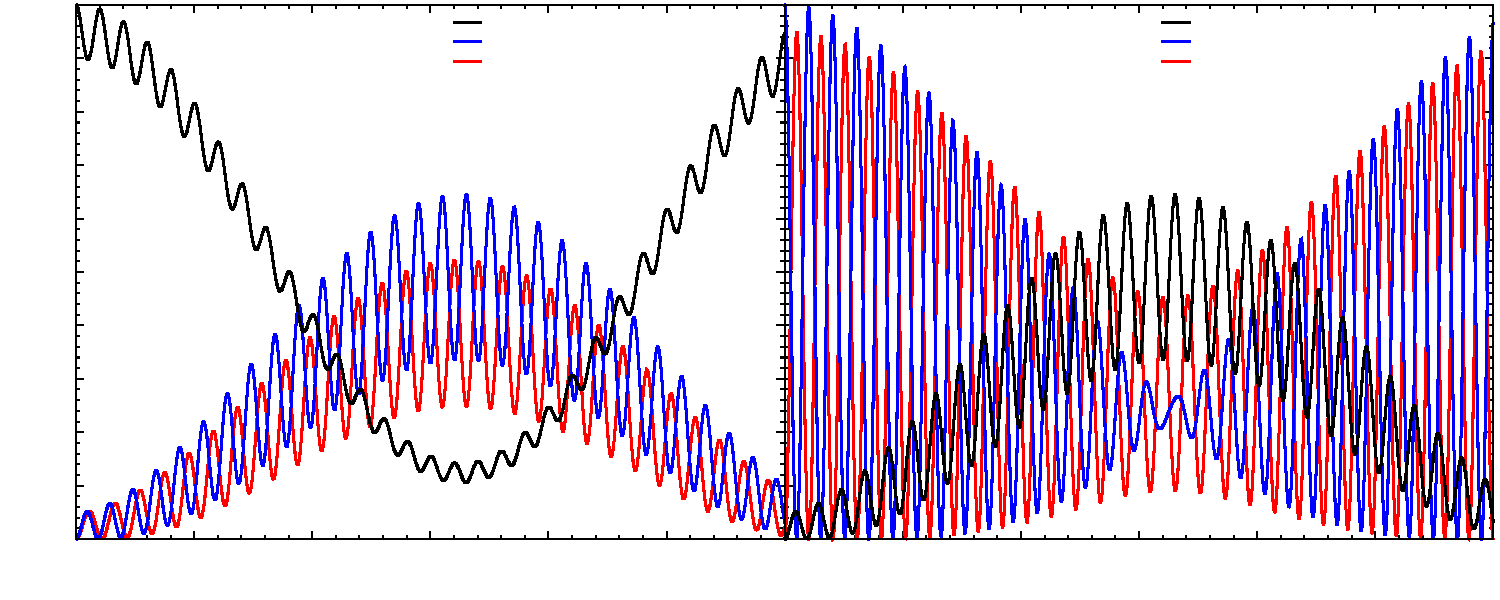
\includegraphics{pics/oscillatorybehave}}%
    \gplfronttext
  \end{picture}%
\endgroup
}
	\caption[Oscillation probability for an initial $\nu_e$ and $\nu_\mu$]%
	{Oscillation probability for an initial $\nu_e$ (left) and $\nu_\mu$ (right), %
	clearly manifesting an oscillatory behaviour with respect to $L/E$.
	The oscillation parameters used here are $\Delta m_{21}^2 = \np{7.6e-5}$\,eV\tapi{2}, %
	$\Delta m_{32}^2 = \np{2.4e-3}$\,eV\tapi{2}, $\sin^2 \theta_{12} = 0.32$, %
	$\sin^2 2\theta_{13} = 0.1$, $\sin^2\theta_{23} = 0.5$, and $\delta_\text{CP} = 0$.}
	\label{fig:osc_behave}
\end{figure}


The oscillating term is the result of the interference of different massive neutrinos, %
which propagate at different velocities, but coherency between states is preserved.
It could happen that neutrinos are produced or detected incoherently, for which interference terms %
do not appear, or that the resolution on the propagation length or the energy is limited, %
for which the probability must be averaged.
In both cases, the oscillation probability simplifies to
\begin{equation}
	\label{eq:average_oscillation}
	\langle P(\nu_\alpha \to \nu_\beta)\rangle = \sum_{i} |U_{\alpha i}|^2 |U_{\beta i}|^2\ ,
\end{equation}
and for $\alpha \neq \beta$ it can be shown that the maximum value the averaged probability %
can take is 
\begin{equation}
	\langle P(\nu_\alpha \to \nu_\beta)\rangle_\text{max} = \frac{1}{N}\ ,
\end{equation}
with $N$ the number of massive neutrinos.
Under these circumstances, the mixing matrix behaves as if its entries have all the same absolute value, %
in an eventuality called \emph{N-maximal mixing}.
This corresponds to minimal average disappearance probability and maximal %
average appearance probability, equal to $1/N$ in each possible channel.

Apart from this limit scenario, the PMNS matrix---and the CKM matrix---are generic %
unitary $N \times N$ matrices, where $N$ is the number of fermion generations.
A matrix with this characteristics depends on $N^2$ independent real parameters, divided among 
\begin{equation}
	\frac{N(N-1)}{2} \quad \text{mixing angles and} \quad
	\frac{N(N+1)}{2} \quad \text{phases}\ ,
\end{equation}
even though, not all the phases are observables, or give physical effects.
Due to the unitarity of the neutral currents, only the weak charged current can manifest these phases, %
despite that $2N-1$ phases can be reabsorbed by a redefinition of the fermion fields.
Excluding the CC term, the SM Lagrangian is invariant under a global phase transformation %
of the lepton and quark fields, such as
\begin{equation}
	\ferm_\alpha \longmapsto e^{i \phi_\alpha^\ferm} \ferm_\alpha\ .
\end{equation}
Let us apply this to the CC current of \refeq{eq:lepton_cc_lagrangian}.
A common phase can be factorised outside
\begin{align}
	%\label{eq:real_quark_cc}
	j^\mu_\text{CC,L}&= 2 \sum_{i = 1}^3 \sum_{\alpha = e, \mu, \tau} %
			    \cj{\nu}_{L i}\, \gamma^\mu e^{-i\varphi_i^\nu} \, V_{\alpha i}^*\, e^{i \varphi_\alpha^\ell} \ell_{L\alpha} \\
			 &= 2 e^{-i (\varphi_3^\nu - \varphi_\tau^\ell)} \sum_{i = 1}^3 \sum_{\alpha = e, \mu, \tau} %
			    \cj{\nu}_{L i}\, \gamma^\mu e^{-i(\varphi_i^\nu - \pi_3^\nu)} \, V_{\alpha i}^*\, %
			    e^{i (\varphi_\alpha^\ell - \varphi_\tau^\ell)} \ell_{L\alpha} \ ,
\end{align}
showing that there are only $2 N -1$ phases that can be reabsorbed in a redefinition of the fields.
A common rephasing would leave the charged current unchanged.
It follows that the number of physical phases is
\begin{equation}
	\frac{N(N+1)}{2} - 2N +1 = \frac{(N-1)(N-2)}{2}
\end{equation}
and so the total physical parameters are
\begin{equation}
	\frac{N(N-1)}{2} + \frac{(N-1)(N-2)}{2} = (N-1)^2 \ .
\end{equation}
In the case of three generations, the PMNS matrix---and the CKM matrix---can be described by three mixing angles %
and just one physical phase.
From a model building point of view, the complex phase may arise from complex Yukawa couplings %
and/or from a relative phase in the vacuum expectation values of Higgs fields.
The PMNS matrix is typically parameterised as follows
%\vspace{-0.2em}
\begin{equation}
	\label{eq:pmns}
	U = \mqty( 1 & 0 & 0 \\ 0 & c_{23} & s_{23} \\ 0 & -s_{23} & c_{23} ) %
	\mqty( c_{13} & 0 & s_{13}e^{-i\delta_\text{CP}} \\ 0 & 1 & 0 \\ -s_{13}e^{i\delta_\text{CP}} & 0 & c_{13} ) %
	\mqty( c_{12} & s_{12} & 0 \\ -s_{12} & c_{12} & 0 \\ 0 & 0 & 1 )\ , %
	%\mqty( 1 & 0 & 0 \\ 0 & e^{i\gamma_1} & 0 \\ 0 & 0 & e^{i\gamma_2} ) %
%\vspace{-0.2em}
\end{equation}
where $c_{ij} \equiv \cos\theta_{ij}$ and $s_{ij} \equiv \sin\theta_{ij}$.
The angle $\delta_\text{CP}$ is the physical phase responsible for CP violation (see \refsec{sec:cp_oscillation}).
It is important to note that if neutrinos were Majorana fermions, there would be two additional %
physical phases and the mixing matrix would contain an extra contribution:
\begin{equation}
	U' = U \ \mqty( 1 & 0 & 0 \\ 0 & e^{-i \gamma_1} & 0 \\ 0 & 0 & e^{-i\gamma_2} ) \ ,
\end{equation}
where $U$ is the same matrix of \refeq{eq:pmns}.
However, due to the structure of the oscillation probability in \refeq{eq:oscillation_probability} %
the Majorana phases do not contribute to neutrino oscillation.
The CKM matrix can be parameterised in an analogous way.

\begin{table}
	\small
	\centering
	\caption[Best fit values for neutrino oscillation parameters]{Best fit values for neutrino oscillation parameters~\cite{Esteban:2018azc}.
		This result includes Super-Kamiokande data and assumes a normal mass ordering.}
	\label{tab:nufit}

	\begingroup
	\def\arraystretch{1.5}%  1 is the default, change whatever you need
	\begin{tabular}{lrr}
		\toprule
		Parameter	& Value		& Error	\\
		\midrule
		$\sin^2 \theta_{12}$	& 0.310		& ${}^{+0.013}_{-0.012}$ 	\\
		$\sin^2 2\theta_{13}$	& 0.0875	& ${}^{+0.0025}_{-0.0025}$	\\
		$\sin^2\theta_{23}$	& 0.563		& ${}^{+0.018}_{-0.024}$	\\
		$\delta_\text{CP} / \pi$			& -0.772 & ${}^{+0.217}_{-0.156}$	\\
		\midrule
		$\Delta m_{21}^2 / \np{e-5}$\,eV\tapi{2}	& 7.39	& ${}^{0.21}_{-0.20}$ 	\\
		$|\Delta m_{32}^2| / \np{e-3}$\,eV\tapi{2}	& 2.528	& ${}^{+0.029}_{-0.031}$ 	\\
		\bottomrule
	\end{tabular}
	\endgroup
\end{table}

The best known value of the mixing angles and mass squared differences are reported in \reftab{tab:nufit}.
The $\delta_\text{CP}$ phase has not been determined as well as the other oscillation angles, %
and synergies between current experiments are used to get the best estimates, before %
next-generation experiments start operation (see \refsec{cha:cp_hk}).
Only one of the two independent squared mass differences is known with its relative sign and %
it is the so-called \emph{solar mass difference} $\Delta m_{21}^2$.
The absolute value of the other mass difference $|\Delta m_{32}^2|$, %
known as \emph{atmospheric mass difference}, has a best value fit which depends on the assumed sign~\cite{Esteban:2018azc}.
If the atmospheric mass difference is positive, then the order between masses is $m_1 < m_2 \ll m_3$, %
otherwise the order is $m_3 \ll m_1 < m_2$.
The first scenario is referred to as \emph{normal hierarchy}, whereas the second one as \emph{inverted hierarchy}.
At first order, it is not possible to extract the hierarchy information from a measurement of neutrino oscillation in vacuum, %
using simply \refeq{eq:oscillation_probability}.
The sign of $\Delta m_{21}^2$ is accessible thanks to the matter effects on the propagation of solar neutrinos.
For the Sun--Earth baseline, the oscillation probability is more sensitive to the solar mass difference, since %
\begin{equation}
	\frac{|\Delta m_{21}^2|}{2} \frac{L}{E} \sim \pi\ ,
\end{equation}
and solar neutrino experiments have constrained $\Delta m_{21}^2 \cos 2\theta_{12} > 0$ (see \refsec{sec:neutrino_matter});
by convention the octant of $\theta_{12}$ is fixed to have $\Delta m_{21}^2 > 0$.
The existing data is not sufficient to determine the sign of the atmospheric mass difference, 
the knowledge of which would define the neutrino mass hierarchy.



\subsection{Propagation of neutrinos in matter}
\label{sec:neutrino_matter}

Neutrinos propagating in a dense medium can interact with its particles, %
although the probability of an incoherent inelastic scattering is very small (see \refsec{sec:neutrino_interactions}).
For example the characteristic cross-section for $\nu$-neutron elastic scattering is of the order
\begin{equation}
	\sigma \simeq \frac{G_F^2 E_\nu^2}{\pi} \sim \np{e-43} \text{cm}^2 \qty(\frac{E_\nu}{\text{MeV}})^2
\end{equation}
where $E_\nu$ is the neutrino energy and $G_F$ is the Fermi constant introduced in \refeq{eq:fermi_const}.
The mean free path of a neutrino passing through a material with number density $n$ can %
be approximated as
\begin{equation}
	\ell \sim \frac{1}{n\,\sigma}\ ,
\end{equation}
assuming the target particles are at rest.
In matter, the main targets are nucleons with mass $m \simeq 1$\,GeV.
If the number density is $n \simeq \mathcal{N}_A$\,cm\tapi{-3}, the mean free path is
\begin{equation}
	\ell \sim \frac{\np{e14}\,\text{cm}^3}{(E/\text{GeV})}\ .
\end{equation}
The Earth, with a diameter of $\sim\np{e9}$\,cm is opaque only to neutrinos with energies above 100\,TeV.
On the other hand, solar neutrinos with energies of the order of 0.1\,MeV have a mean free path through %
matter of 0.1 light years.
The interaction rate changes significantly in materials with a very high number density, %
such as in neutron stars or supernovae.
It was first noted in \refref{Wolfenstein:1977ue} that neutrinos propagating in dense regions are subject %
to an effective potential due to the coherent forward elastic scattering with the particles in the medium.
%When neutrinos propagate in dense matter, they can also interact coherently with the particles in the medium.
In coherent interactions it still is possible to have interference between the scattered and the unscattered neutrino waves %
which enhances the effect of matter in the neutrino propagation.
Differently from vacuum interference, in this case the effect of the medium is not on the intensity %
of the propagating neutrino beam, which remains unchanged, but on the phase velocity of the wave packets.
The phenomenon can be seen as a refractive index that modifies the mixing of neutrinos.
%For this reason the effect is proportional to $G_F$, %
%instead of the $G_F^2$ dependence of the incoherent scattering.
%Coherence also allows decoupling the evolution equation of the neutrinos from those of the medium.
%In this limit the effect of the medium is introduced in the evolution equation for the neutrinos %
%in the form of an effective potential which depends on the density and composition of the matter.

The forward scattering possible for neutrinos in matter are CC interactions of %
$\nu_e$ on electrons and NC interactions of any neutrino on electron, protons, and neutrons.
The effective four-point Hamiltonians for these interactions (see \refeqs{eq:fermi_cc}{eq:fermi_nc}) %
are, up to Fierz re-ordering, 
\begin{align}
	\mathcal{H}_\text{CC} &= \frac{G_F}{\sqrt{2}} \qty[\cj{\nu}_e \gamma^\mu(1-\gamma^5)\nu_e] %
		 	      				\qty[\cj{e}\,\gamma_\mu(1 - \gamma^5) e]\ , \\
	\mathcal{H}_\text{NC} &= \frac{G_F}{\sqrt{2}} \sum_{\alpha=e, \mu, \tau} %
							\qty[\cj{\nu}_\alpha \gamma^\mu(1-\gamma^5)\nu_\alpha] %
							\sum_{\ferm = e, p, n} \qty[\cj{\ferm}\,\gamma_\mu(g^F_V - g^F_A \gamma^5) \ferm]\ .
\end{align}
The fermions, either electrons, neutrons, or protons, must have identical four-momenta and helicities %
in their initial and final states, thanks to the coherent nature of the scattering.
Let us therefore average the effective Hamiltonian on the fermion background using %
a statistical distribution $\rho$ of the fermion energy at a given temperature of the medium, %
which normalises to the total number of particles
\begin{equation}
	N_\ferm = \int \dd[3]{p} \rho(E_\ferm, T) \ .
\end{equation}
Finally, averaging over the helicities of the fermions, terms proportional to the current are obtained
\begin{align}
	\expval{\mathcal{H}_\text{CC}} &= V_\text{CC}\, \cj{\nu}_{eL} \gamma^0 \nu_{eL}\ , \\
	\expval{\mathcal{H}_\text{NC}} &= \sum_{\ferm = e, p, n} V^\ferm_\text{NC} %
					 \sum_{\alpha=e, \mu, \tau} \cj{\nu}_{\alpha L} \gamma^0\nu_{\alpha L} \ ,
\end{align}
where the effective potentials are
\begin{align}
	V_\text{CC} &= \sqrt{2}\,G_F\, n_e\ , \\
	V^\ferm_\text{NC} &= \sqrt{2}\,G_F\, n_\ferm\,g_V^\ferm \ .
\end{align}
The vector coupling constants for electrons and protons are equal and opposite
\begin{equation}
	g_V^e = -g_V^p = -\frac{1}{2} + 2 \sin^2 \vartheta_\text{W}\ ,
\end{equation}
but due to the neutrality of matter the densities have the same value, i.e.\ $n_e = n_p$, %
and so their NC contributions cancel out.
Neutrons are the only particles providing an overall potential to neutrino neutral-current interactions %
and since they are chargeless  the corresponding potential is
\begin{equation}
	V_\text{NC} = -\frac{\sqrt{2}}{2} G_F\,n_\ferm \ .
\end{equation}

The total Hamiltonian is $\mathcal{H} = \mathcal{H}_0 + \mathcal{H}_\text{m}$, %
where $\mathcal{H}_0$ is the Hamiltonian in vacuum (see \refeq{eq:hamilton}).
The operator $\mathcal{H}_\text{m}$ acts on neutrino flavour state as
\begin{equation}
	\label{eq:ham_mat}
	\mathcal{H}_\text{m} \ket{\nu_\alpha} = V_\alpha \ket{\nu_\alpha}\ ,
\end{equation}
and the total potential is defined as
\begin{equation}
	V_\alpha = V_\text{CC} \delta_{\alpha e} + V_\text{NC} = %
		   \sqrt{2}\,G_F \qty( n_e \delta_{\alpha e} - \frac{1}{2} n_n)\ .
\end{equation}
The massive neutrino states are eigenstates of the free Hamiltonian, but %
for $\mathcal{H}_m$ the description in the flavour basis is simpler.
It is convenient to define the transition amplitude 
\begin{equation}
	\phi_{\alpha \beta} (t) = \braket{\nu_\beta}{\nu_\alpha (t)}\ ,
\end{equation}
from which the transition probability is simply
\begin{equation}
	P(\nu_\alpha \to \nu_\beta) = \qty|\phi_{\alpha \beta} (t)|^2\ .
\end{equation}
From \refeqs{eq:hamilton}{eq:ham_mat}, it follows that 
\begin{equation}
	\mathcal{H}\ \phi_{\alpha \beta} (t) = %
		\sum_\rho \qty(\sum_i U_{\beta i} E_i U^*_{\rho i} + \delta_{\beta \rho} V_\beta)\,
		\phi_{\alpha \rho} (t)\ .
\end{equation}
With this relation, the propagation of neutrinos in matter can be derived in complete analogy with the oscillation in vacuum.
The evolution of neutrino states in time comes from solving the Schr{\"o}dinger's equation and %
the probability of flavour transition can be computed.
Using the same approximations introduced for vacuum oscillations, the evolution equation becomes
\begin{equation}
	i \dv{}{x} \phi_{\alpha \beta}(x) = %
		\sum_\rho \qty(\sum_i\frac{\Delta m_{i1}^2}{2E}  U_{\beta i} U^*_{\rho i} + %
			\delta_{\beta e} \delta_{\rho e} V_\text{CC}) \phi_{\alpha \rho} (x)\ .
\end{equation}
The term
\begin{equation}
	p + \frac{m_1^2}{2E} + V_\text{NC} \phi_{\alpha \beta}(x)
\end{equation}
has been removed, since it generates a common phase to all flavours and so it is irrelevant to flavour transitions.

The treatment of oscillations in matter for three-neutrino mixing can be quite intricate, %
because of the combinations between the different mass squared differences.
%Fortunately, in the case of the hierarchy of squared-mass differences, for which
%\begin{equation}
%	\label{eq:hierarchy}
%	\Delta m^2_\text{sol} = \Delta m^2_{21} \ll \Delta m^2_\text{atm} = |\Delta m^2_{31}|\ ,
%\end{equation}
%the effects of the large and small squared-mass differences can be separated out, %
%leading to a considerable simplification of the following discussion.
%and a clear understanding of the physical mechanisms at work in experiments.
Let us consider a simpler scenario of only two neutrino generations, $\nu_e$ and $\nu_\mu$.
Assuming the initial flavour being $\alpha = e$, the evolution equation is now 
\begin{align}
	i \dv{}{x} \mqty(\phi_{e e} \\ \phi_{e \mu}) &= %
			\mathcal{H}_F \mqty(\phi_{e e} \\ \phi_{e \mu}) \notag \\
	\label{eq:two_flav_evolution}
		&= \frac{1}{4E} \mqty( -\Delta m^2 \cos 2\theta + A_\text{CC} & \Delta m^2 \sin 2\theta \\
				    \Delta m^2 \sin 2\theta	& \Delta m^2 \cos 2\theta - A_\text{CC} ) %
		   \mqty(\phi_{e e} \\ \phi_{e \mu})\ ,
\end{align}
where $\Delta m^2 = m_2^2 - m_1^2$ and $\theta$ is the mixing angle, as in
\begin{equation}
	\mqty(\nu_e \\ \nu_\mu)  =
		\mqty ( \cos \theta & \sin \theta \\ -\sin\theta & \cos\theta ) %
	\mqty(\nu_1 \\ \nu_2)\ ,
\end{equation}
and 
\begin{equation}
	A_\text{CC} \equiv 2 \sqrt{2} E\,G_F\,n_e\ .
\end{equation}
The effective Hamiltonian $\mathcal{H}_F$ of \refeq{eq:two_flav_evolution} can be diagonalised by means of %
an orthogonal transformation
\begin{equation}
	O_M = \mqty ( \cos \theta_M & \sin \theta_M \\ -\sin\theta_M & \cos\theta_M )\ ,
\end{equation}
to obtain 
\begin{equation}
	\mathcal{H}_M = O_M^T \mathcal{H}_F O_M = \frac{1}{4E} \text{diag} (-\Delta m^2_M, \Delta m^2_M)\ .
\end{equation}
The effective mixing angle $\theta_M$ is given by
\begin{equation}
	\tan 2\theta_M = \frac{\tan 2\theta}{1 - \displaystyle\frac{A_\text{CC}}{\Delta m^2 \cos 2\theta}}
\end{equation}
and the effective mass squared difference $\Delta m_M^2$ reads
\begin{equation}
	\qty(\Delta m^2_M)^2 = (\Delta m^2 \cos 2\theta - A_\text{CC})^2 + (\Delta m^2 \sin\theta)^2\ .
\end{equation}
It was found in \refrefs{Mikheev:1986gs, Mikheev:1986wj} that it is possible to have a resonant flavor transitions %
when neutrinos propagate in a medium with varying density, with the effective mixing angle %
passing through the maximal mixing value of $\pi/4$.
This resonance condition is achieved when 
\begin{equation}
	A_\text{CC} = \Delta m^2 \cos2\theta\ ,
\end{equation}
or equivalently
\begin{equation}
	n_e = \frac{\Delta m^2 \cos2\theta}{2\sqrt{2} E\,G_F }\ .
\end{equation}
Transforming the transition probability to the mass basis by means of $O_M$, %
the evolution equation becomes
\begingroup
\renewcommand*{\arraystretch}{1.25}
\begin{equation}
	\label{eq:two_flav_evolution_diag}
	i \dv{}{x} \mqty(\phi'_{e 1} \\ \phi'_{e 2}) = %
		\mqty(\displaystyle -\frac{\Delta m^2_M}{4E}  &\displaystyle -i \dv{\theta_M}{x}  \\
		\displaystyle i \dv{\theta_M}{x}  &\displaystyle \frac{\Delta m^2_M}{4E}) %
		   \mqty(\phi'_{e 1} \\ \phi'_{e 2})\ .
\end{equation}
\endgroup
It is interesting to note that if the matter profile is constant, then $\dv*{\theta_M}{x} = 0$ %
and the structure of the oscillation probability simplifies to a two-flavour oscillation in vacuum, %
with effective mixing angle $\theta_M$ and mass squared difference $\Delta m^2_M$.
On the other hand, if the matter density is not constant, the variation of $\theta_M$ %
must be taken into account.
It reads
\begin{equation}
	\dv{\theta_M}{x} = \frac{\sin 2\theta_M}{2\Delta m^2} \dv{A_\text{CC}}{x}\ .
\end{equation}
If the variation of the effective matter angle is small compared to the diagonal terms of %
the Hamiltonian of \refeq{eq:two_flav_evolution_diag}, then the transition %
between neutrino mass states in matter is negligible.
With the condition
\begin{equation}
	\label{eq:adiabaticity}
	\frac{\Delta m_M^2}{4E}\, \qty|\dv{\theta_M}{x}|^{-1} = %
	\frac{(\Delta m_M^2)^2}{2E\ \sin2\theta_M}\, \qty|\dv{A_\text{CC}}{x}|^{-1} \gg 1
\end{equation}
satisfied along the neutrino path, the transition is said to be \emph{adiabatic} %
and flavour conversion occurs without oscillation between states.

The condition of adiabaticity is typically met for solar and supernova neutrinos, %
for which the medium profile smoothly changes from the high density of the core %
to the vacuum or the density of the detector, which is practically negligible.
Neutrinos are produced in astrophysical sources mostly in the electron flavour (see \refsec{sec:nu_prod}).
Regarding terrestrial experiments, the distance between the source and the detector is much larger than %
the detector itself, which means that only the averaged probability can be measured.
If at production the matter potential is well-below the resonance value, i.e.\ $A_\text{CC} \ll \Delta m^2 \cos\theta$, %
the matter effects are negligible and the propagation occurs almost in vacuum with an average survival probability
\begin{equation}
	\expval{P(\nu_e\to\nu_e)} = 1 - \frac{1}{2} \sin^2 2\theta\ .
\end{equation}
If the matter potential at production is closer to the resonant potential, i.e.\ $A_\text{CC} \lesssim \Delta m^2 \cos\theta$, %
the resonance is not crossed, but the propagation can be still described by an adiabatic propagation.
The survival probability is  now
\begin{equation}
	\label{eq:avg_probability_matter}
	\expval{P(\nu_e\to\nu_e)} = \frac{1}{2} + \frac{1}{2} \cos 2\theta_M \cos2\theta\ ,
\end{equation}
where $\theta_M$ is the effective mixing angle in matter at the production point.
Since the resonance condition is not met, $\cos\theta_M$ has the same sign of $\cos\theta$ and %
so $\expval{P(\nu_e\to\nu_e)} > \flatfrac{1}{2}$.
When the potential is such that $A_\text{CC} \gtrsim \Delta m^2 \cos\theta$, the resonance can be crossed %
and this occurs if $\cos2\theta > 0$, assuming $\Delta m^2 > 0$.
It follows that the produced neutrino $\nu_e$ has a larger component of $\nu_2$ in matter, %
but when in vacuum the main component becomes $\nu_1$.
Finally, if the density is much higher than the resonance one, i.e.\  $A_\text{CC} \gg \Delta m^2 \cos\theta$, %
the effective mixing angle in matter is maximal, $\theta_M \simeq \flatfrac{\pi}{2}$, %
and so the $\nu_e$ is produced mostly as $\nu_2$.
As the neutrino travels to regions of lower density crossing the resonance adiabatically, %
the final mixing angle in matter tends to the mixing angle in vacuum and %
so $\nu_2 = \sin\theta \nu_e + \cos\theta \nu_\mu$.
If the vacuum angle $\theta$ is small, the overall effect is a smooth conversion from $\nu_e$ to $\nu_\mu$.
The survival probability becomes the same of \refeq{eq:avg_probability_matter} and %
this mechanism is known as Mikheyev-Smirnov-Wolfenstein (MSW) effect.
When the condition of adiabaticity is violated, there might be transition between the two neutrino mass states in matter.
The expression in \refeq{eq:adiabaticity} gets its minimum value with
\begin{equation}
	\dv[2]{\cos2\theta}{x} = 0\ ,
\end{equation}
and the survival probability is modified into~\cite{Parke:1986jy}
\begin{equation}
	\label{eq:parke_probability_matter}
	\expval{P(\nu_e\to\nu_e)} = \frac{1}{2} + \qty(\frac{1}{2} - P_{12}) \cos 2\theta_M \cos2\theta\ ,
\end{equation}
where $P_{12}$ is the crossing transition probability between the two states $\nu_1$ and $\nu_2$ at the resonance. 
The adiabatic case is recovered when $P_{12} = 0$.

\section{Neutrino production}
\label{sec:nu_prod}

Neutrinos are the most abundant fermions in the Universe.
With the expansion and cooling of the Universe, the interaction rate of primordial neutrinos %
decreased below the expansion rate, resulting in a decoupling of the neutrinos from the other particles.
These \emph{relic neutrinos} form what is called the Cosmic Neutrino Background (C$\nu$B), %
a radiation analogous to the Cosmic Microwave Background (CMB) which also decoupled at the early stages of the Universe.
The C$\nu$B formed well before the CMB, due to the weak nature of neutrino interactions, %
and it has a temperature given by the relation
\begin{equation}
	\label{eq:nu_temperature}
	T_\nu = \qty(\frac{4}{11})^{\flatfrac{1}{3}} T_\gamma = (\np{1.945} \pm \np{0.001})\,\text{K}\ .
\end{equation}
This relation makes a precise prediction of the temperature of the neutrinos $T_\nu$, %
connecting it with the photon temperature $T_\gamma$, which is accurately measured by CMB surveys.
The temperature is equivalent to $T_\nu = (\np{1.676} \pm \np{0.001}) \times 10^{-4}$\,eV.
By comparing this energy to the measured mass differences from oscillation experiments (see \refsec{tab:nufit}) %
one can infer that at least two mass states of relic neutrinos are non-relativistic.
However, neutrinos at the these energies are almost impossible to detect with the current technologies and it will be a challenge %
for next-generation experiments.

The density of relativistic neutrinos can be related to the density of photons, thanks to \refeq{eq:nu_temperature} %
by which
\begin{equation}
	\label{eq:nu_gamma_density}
	\frac{\rho_\nu}{\rho_\gamma} = \frac{7}{8} \qty(\frac{4}{11})^{\flatfrac{1}{3}} N_\text{eff}\ ,
\end{equation}
and so the energy density with respect to the critical density is
\begin{equation}
	\label{eq:rel_density}
	\Omega_{\nu_\text{R}}\, h^2 = \qty(\frac{4}{11})^{\flatfrac{1}{3}} \Omega_\gamma\, h^2\ ,
\end{equation}
with $h$ the Hubble constant.
When the neutrinos are non-relativistic, their energy density is given by $\rho_\nu \simeq \sum_i m_i n_i$, %
where $n_i$ are the number density of each species which are equal to each other, %
up to negligible corrections from flavour effect.
Using the expression of \refeq{eq:nu_gamma_density} and knowing the number density of photons $n_\gamma$, %
the total energy density of non-relativistic neutrinos today is
\begin{equation}
	\label{eq:nonrel_density}
	\Omega_{\nu_\text{NR}}\, h^2 = \frac{\sum_i m_i}{\np{94.14}\,\text{eV}}\ ,
\end{equation}
and the contribution of relativistic neutrinos to the total mass is also negligible.
Due to the fact that the density from \refeq{eq:nonrel_density} can never be greater than %
the energy density of all matter in the Universe, a naive bound on the neutrino masses can be derived:
\begin{equation}
	\sum_i m_i \lesssim 13\,\text{eV}\ .
\end{equation}
The limit can be improved with more precise theoretical considerations under $\Lambda$CDM assumption %
which combined with the latest cosmological surveys goes down to $\sum_i m_i \lesssim 0.12$~\cite{Giusarma:2013pmn}.

Other than cosmological neutrinos, these elusive fermions are produced and involved in a large variety of processes.
They are emitted in astrophysical processes, such as supernova explosions, blazars, and in the nuclear reactions %
of the cores of stars.
Cosmic ray interactions with the Earth's atmosphere also produce neutrinos from decays of secondary mesons.
Human-made sources include accelerator facilities in which neutrino beams are produced in a controlled environment, %
as well as those emitted by nuclear reactors.
Neutrinos are also the products of natural-occurring $\beta$-decays, from the study of which neutrinos were first hypothesised. 
The study of the rare double-$\beta$ decay is of utter importance, % 
because the proposed neutrinoless manifestation of this decay is a true lepton number violating process, %
the detection of which has deep and considerable connotations for neutrino mass theories~\cite{Majorana:1937vz}.

In the following sections the most relevant sources for the neutrino experiment mentioned in this thesis are discussed.

\subsection{Solar and supernova neutrinos}
\label{sec:nu_sun_sn}

\begin{table}
	\small
	\centering
	\captionof{table}[Processes emitting $\nu_e$ in the $pp$ chain and the CNO cycle]%
		{Processes occurring in the $pp$ chain (left) and the CNO cycle (right) that emit $\nu_e$.
		The first column of the $pp$ chain table lists the typical label with which the %
		processes are referred to; the neutrinos of the CNO cycle are labelled with the name of the decaying nuclide. 
		In both tables, the maximum neutrino energy is also reported.}
	\label{tab:pp_cno}

	\begin{tabular}{lr@{~$\longrightarrow$~}lr}
		\toprule
		\raisebox{0.6em}{Label}	& \multicolumn{2}{c}{\raisebox{0.6em}{Process}}	& \shortstack{$E_\text{max}$ \\ (MeV)} 	\\
		\midrule
		$\bs{pp}$	    & $p + p$		 & \tapi{2}H $+ e^+ + \nu_e$		& 0.423 \\
		$\bs{pep}$	    & $p + e^- + p$	 & \tapi{2}H $+ \nu_e$			& 1.445 \\
		$\bs{hep}$	    & \tapi{3}He $+ p$   & \tapi{4}He $+ e^+ + \nu_e$		& 18.778 \\
		\textbf{\tapi{7}Be} & \tapi{7}Be $+ e^-$ & \tapi{7}Li $+ \nu_e$			& 0.386 \\
		\textbf{\tapi{8}Be} & \tapi{8}Be	 & \tapi{8}Be\tapi{*} $+ e^+ + \nu_e$	& 0.862 \\
				    &			 & 2\,\tapi{4}He $+ e^+ + \nu_e$ 	& $\sim$15 \\
		\bottomrule
	\end{tabular}
	\hfill
	\raisebox{1.85em}{
	\begin{tabular}{r@{~$\longrightarrow$~}lr}
		\toprule
		 \multicolumn{2}{c}{\raisebox{0.6em}{Process}}	& \shortstack{$E_\text{max}$ \\ (MeV)} 	\\
		\midrule
		\tapi{13}N    & \tapi{13}C $+ e^+ + \nu_e$ & 1.198\,MeV \\
		\tapi{15}O    & \tapi{15}N $+ e^+ + \nu_e$ & 1.732\,MeV \\
		\tapi{17}F    & \tapi{17}F $+ e^+ + \nu_e$ & 1.736\,MeV \\
		\bottomrule
	\end{tabular}}
\end{table}

Neutrinos emitted by the Sun were the first astrophysical source of neutrinos detected.
They are produced by thermonuclear reactions occuring in the solar core.
Being a G-type star in the main sequence, the Sun is powered mostly from proton--proton chain ($pp$) %
and partly by the carbon--nitrogen--oxygen cycle (CNO).
In both these processes, the net result is the conversion of four protons and two electrons into an $\alpha$-particle %
and two electron neutrinos
\begin{equation}
	\label{eq:sun_net}
	4\,p\ +\ 2\,e^- \longrightarrow {}^4\text{He}\ +\ 2\, \nu_e\ ,
\end{equation}
along with the release of $\np{26.731}$\,MeV in the form of photons or kinetic energy of the neutrinos.
The processes of the $pp$ chain and CNO cycle releasing neutrinos are reported in \reftab{tab:pp_cno}.
Due to their elusive nature and low energy, solar neutrinos are difficult to detect in detail and %
therefore a reliable theoretical model describing the solar nuclear reactions is needed.
The standard solar model (SSM), developed by Bahcall and collaborators~\cite{Bahcall:1997ha}, %
perfectly agrees with data from helioseismology~\cite{Bahcall:1987jc}, such as the speed of sound and the density profile of the Sun, %
and for this reason it is considered to provide a credible estimate of the flux of neutrinos produced in the Sun, %
predicted in \reffig{fig:solar_nu_flux}.
The first neutrino experiments, such as Homestake~\cite{Lande:1991np}, GALLEX/GNO~\cite{Altmann:2005ix}, %
and SAGE~\cite{Abdurashitov:2002nt,Abdurashitov:2005tb}, were in strong disagreement with the predictions of the SSM.
The so-called \emph{solar neutrino problem} was later solved by the SNO experiment~\cite{Aharmim:2005gt}, %
which demonstrated the presence of flavour transition, explained theoretically by the MSW effect (see \refsec{sec:neutrino_matter}).
The low-background and low-threshold BOREXINO experiment~\cite{Tartaglia:2001sh} was able to measure different solar neutrinos %
across the energy spectrum reaching good agreement with the theoretical prediction of flavour transition in matter~\cite{Bellini:2014uqa}, %
as shown in \reffig{fig:borex}.

\begin{figure}
	\begin{minipage}[t]{0.48\textwidth}
		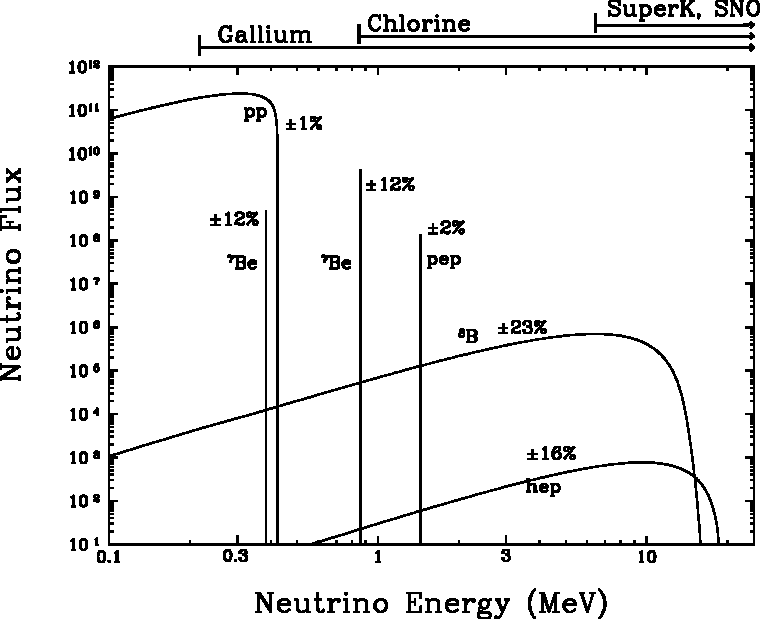
\includegraphics[width=\textwidth]{pics/BahcallNuFlux.pdf}
		\captionof{figure}[Solar standard model prediction of the solar neutrino flux]%
		{The neutrino flux from the $pp$ chain, predicted with the solar standard model~\cite{Bahcall:2004mz}.
		The threshold energies of major solar neutrino experiments are shown for comparison.}
		\label{fig:solar_nu_flux}
	\end{minipage}
	\hfill
	\begin{minipage}[t]{0.5\textwidth}
		\centering
		\raisebox{0.45em}{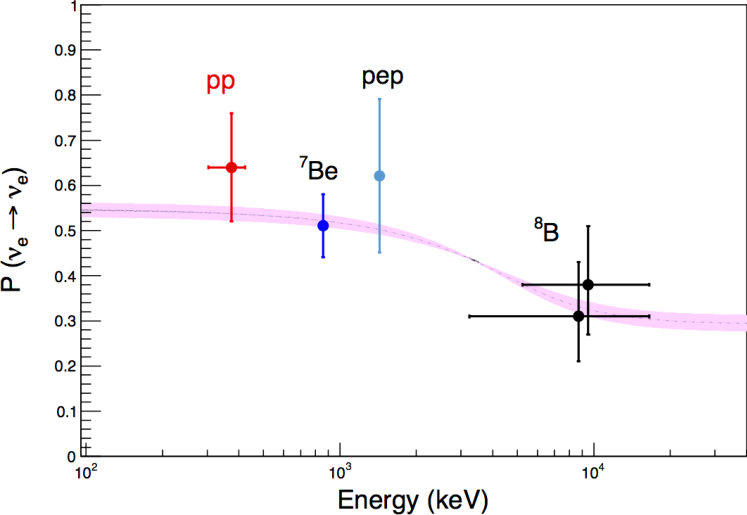
\includegraphics[width=\textwidth]{pics/borexino.pdf}}
		\captionof{figure}[Survival probability of $\nu_e$ measured by BOREXINO]%
		{Survival probability of $\nu_e$ produced by the different nuclear reactions in the $pp$ chain, %
		as measured by BOREXINO~\cite{Bellini:2014uqa}.
		The violet band corresponds to the $\pm1\sigma$ prediction of the flavour transition in the Sun.}
		\label{fig:borex}
	\end{minipage}
\end{figure}


The second astrophysical source of neutrinos ever identified was the Supernova (SN) explosion SN1987A %
which occurred on the 23\tapi{rd} of February, 1987, in the Large Magellanic Cloud.
It was the only SN explosion which was detected through its neutrino burst.
In spite of this fact, supernova explosions are the most intense sources of neutrinos in the Universe.
Historically, SN are classified by their spectral characteristics near maximal luminosity.
This is dictated by the composition of the progenitor star.
The main subdivision is between spectra with or without hydrogen lines, respectively called %
type II and type I.
Further classification of type I SN comes from the presence of silicon and helium.
Type Ia SN, the spectrum of which shows strong Si lines, is the only SN type that is not accompanied %
by a substantial neutrino emission.
This is because the mechanism of explosion comes from the accretion of a white dwarf to the point where %
the pressure of the degenerate electron gas can no longer sustain the gravitational pull.
The limit is known as \emph{Chandrasekhar limit} and it is around 1.4\,$M_\odot$~\cite{Chandrasekhar:1931ih}.
When the white dwarf collapses, the fusion of carbon and oxygen heavy nuclei is activated %
and an enormous quantity of energy is freed in thermonuclear processes.

On the other hand, the supernovae of type Ib and Ic (with He lines) and II explode via a core-collapse, %
liberating an intense flux of neutrinos.
Old stars with a mass $M \gtrsim 8\,M_\odot$ and $M \lesssim 40\,M_\odot$ tend to stratify %
in layers of elements undergoing fusion, with the lightest (H) in the outer shell burning into heavier nuclei %
(He, C, Ne, Mg, Si, ...) up to iron at the core.
After carbon ignition, the neutrino luminosity of the star comes mainly from a long silicon burning phase.
The \emph{pre-supernova} neutrinos from Si fusion make up roughly 1\,\% of the total energy that is emitted during the star's core-collapse.
At this stage, the gravitational pressure is balanced overall by the thermonuclear energy released in each shell, %
but in the Fe core for which exothermic reactions are not allowed.
The mass of the core is sustained by the pressure of degenerate relativistic electrons, %
which is reduced by photodissociation of iron 
\begin{equation}
	\gamma +  {}^{56}\text{Fe} \to 13\,\alpha + 4\,n - 124.4\,\text{MeV}\ ,
\end{equation}
and electron capture with neutrinos escaping the supernova
\begin{equation}
	e^- + p \to n + \nu_e\ .
\end{equation}
Once the Fermi pressure is no longer sufficient to contrast the core, this collapses %
and the increase in temperature accelerates photodissociation and electron capture in a positive feedback reaction.
The density of the core however increases until when neutrinos from electron capture are trapped inside %
and so the collapse becomes an adiabatic process.
The free-falling core is finally stopped by the pressure of degenerate non-relativistic nucleons.
The abrupt halt causes a shock wave that propagates to the outer parts of the core and slows down the imploding mantle.
As the shock propagates through the in-falling dense matter of the outer core,
the energy of the shock is dissipated by the photodissociation of nuclei into nucleons, %
leading to an intensification of the electron capture rate thanks to the copious number of free protons.
The electron neutrinos pile up behind the opaque wave until the shock reaches a layer of lower density 
and the $\nu_e$ are released in a few milliseconds in what is called \emph{neutronisation burst}, %
carrying away around \np{e50}\,erg.
In most scenarios, the shock wave stalls and the bounce mechanism from the core alone is not enough to cause an explosion.
The remnant of the core, which is forming a proto-neutron star, can revive the shock if its mass is large enough.
In the hot core, numerous neutrinos are produced in all flavours by electron-positron annihilation, %
electron-nucleon and nucleon-nucleon bremsstrahlung, and electron neutrinos from electron or positron capture.
These neutrinos remain trapped between the core and the mantle regions with a density high enough such that %
their mean free path is smaller than the supernova radius.
This region, known as \emph{neutrinosphere}, depends on the $\nu$ energies and flavours %
and emits a thermal flux of neutrinos the energy of which is believed to revive the shock up to explosion.
The luminosity of neutrinos in this phase does not peak as for the neutronisation burst, %
but presents a long hump on a time scale of a few seconds, as seen in \reffig{fig:sn_nu_flux}.
The average energies are typically higher for muon and tau neutrinos, since they are produced in deeper %
region of the SN, the values of which strongly depend on the model (see for example \refrefs{Totani:1997vj, Nakazato:2012qf, Tamborra:2014hga}).
The energies for both neutrinos and antineutrinos usually range between 10\,MeV and 30\,MeV.

\begin{figure}
	\centering
	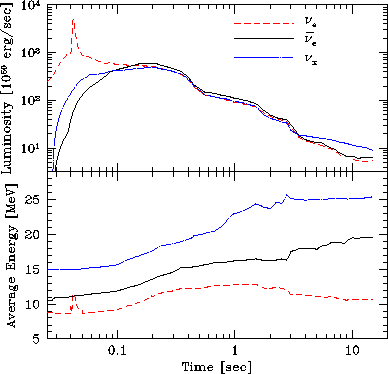
\includegraphics[width=0.5\textwidth]{pics/SN_burst.pdf}
	\caption[Neutrino flux from a core-collapse supernova]%
	{Time and energy profile of the predicted neutrino flux from a Supernova core-collapse of %
	mass $M \simeq 20\,M_\odot$~\cite{Totani:1997vj}.
	Other neutrino flavours than $\nu_e$ and $\cj{\nu}_e$ are collectively represented by %
	$\nu_X = (\nu_\mu + \cj{\nu}_\mu + \nu_\tau + \cj{\nu}_\tau) / 4$.
	From the prediction, the neutronisation burst of $\nu_e$ is visible at early stages of the explosion, %
	whereas neutrinos of all flavours are emitted at later times.}
	\label{fig:sn_nu_flux}
\end{figure}

The estimated rate of Supernova explosions in our Galaxy is relatively low, %
around two to three explosions per century~\cite{Tammann:1994ev}.
Considering the whole Universe however this rate should be much higher.
All core-collapse SN in the causally-connected Universe are isotropically distributed %
and therefore an isotropic and time-independent neutrino flux should exist.
This stochastic flux is known as \emph{Diffuse Supernova Neutrino Background} (DSNB) %
and the detectable neutrinos are called \emph{Supernova Relic Neutrinos} (SRN).
The energy density of SRN is around $0.01$\,eV\,cm\tapi{-3}, which is roughly ten times less %
than that of the CMB, but it is comparable to the density number of all photons from stars.
The energy spectrum should peak at a few MeV, where the inverse beta decay (IBD) interaction %
for $\cj{\nu}_e$ dominates (see \refsec{sec:ccqe}).
This process is the best discovery prospect for SRN in water Cherenkov experiments like Super-Kamiokande, %
thanks to low background and high cross-section in this energy region~\cite{Beacom:2010kk}.
Despite being a challenging task, the detection of the DSNB is fundamental for astrophysics and stellar formation, %
because the study of SN cannot rely just on very rare galactic core-collapse explosions.

\subsection{Atmospheric neutrinos}
\label{sec:nu_atm}

\begin{figure}[t]
	\centering
	%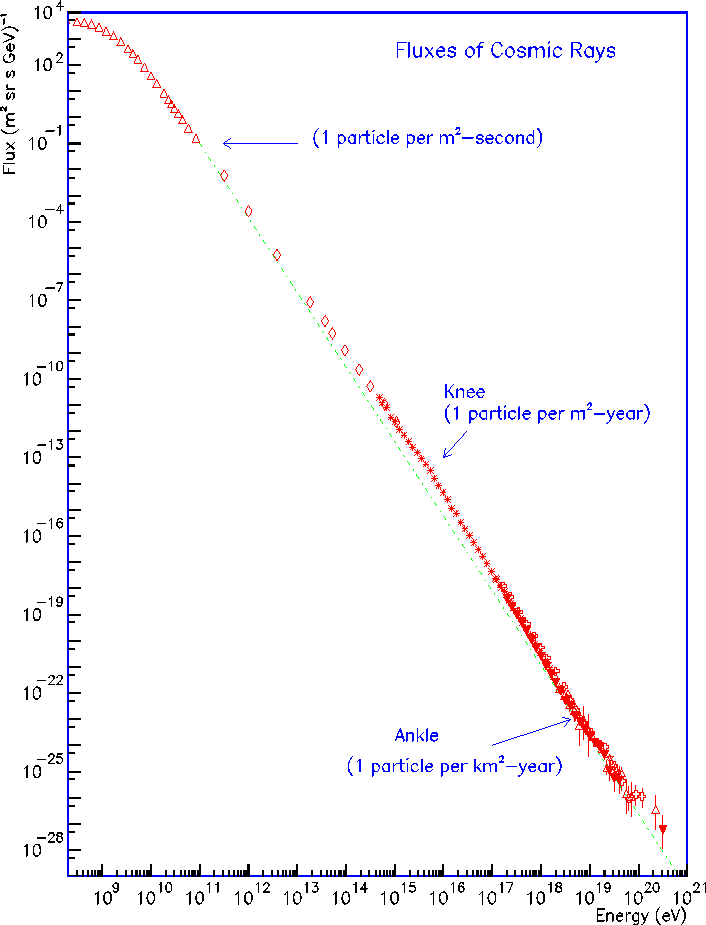
\includegraphics[width=0.9\textwidth]{pics/CR_flux.pdf}
	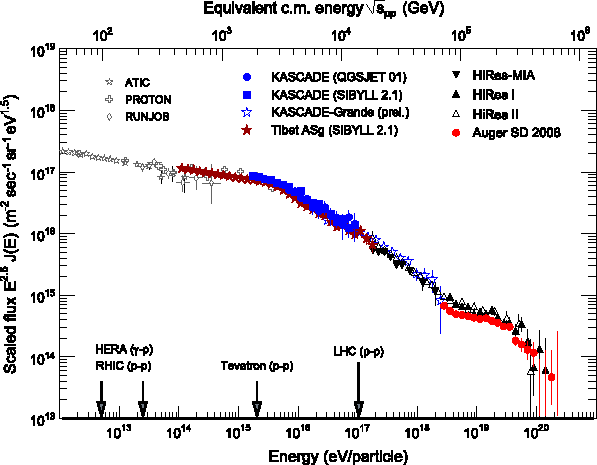
\includegraphics[width=0.7\textwidth]{pics/cosmicrays.pdf}
	\captionof{figure}[Energy spectrum of cosmic rays]%
	{Measurement of cosmic rays over the entire energy spectrum, %
	where the change of energy dependence (\emph{knee}) is visible at around \np{e15}\,eV.
	The flux is multiplied by the power law $E^{2.5}$. Taken from \refref{Bluemer:2009zf}.}
	\label{fig:CR_flux}
\end{figure}

Atmospheric neutrinos are generated by the interactions of cosmic rays with the Earth's atmosphere.
Primary cosmic rays are mainly composed by energetic protons or heavier nuclei, originated from the Sun %
or outside the solar system.
Their interactions with nuclei in the atmosphere produces pseudo-scalar mesons such as pions and kaons, %
which rapidly decay into charged leptons and neutrinos.
Due to helicity suppression, the two-body decays of $\pi^\pm$ and $K^\pm$ favour the muon channel
\begin{align}
	\pi^\pm &\rightarrow \mu^\pm + \overset{(-)}{\nu_\mu}\ , \\
	K^\pm &\rightarrow \mu^\pm + \overset{(-)}{\nu_\mu} \ .
\end{align}
The muon itself decays with a relatively longer lifetime releasing two neutrinos per decay:
\begin{align}
	\mu^+ &\rightarrow e^+ + \nu_e + \cj{\nu}_\mu\ , \\
	\mu^- &\rightarrow e^- + \cj{\nu}_e + \nu_\mu \ .
\end{align}
At sufficient low energies around $E \lesssim 1$\,GeV, all of the muons decay before reaching the ground and %
so the neutrino fluxes follow the proportions of neutrino flavours 
\begin{align}
	\phi_{\nu_e} : \phi_{\nu_\mu} &= 1 : 2 \ ,\\
	\phi_{\nu_\mu} : \phi_{\cj{\nu}_\mu} &= 1 : 1\ , \\
	\phi_{\nu_e} : \phi_{\cj{\nu}_e} &= \phi_{\mu^+} : \phi_{\mu^-} \ .
\end{align}
At higher energies, the amount of muons hitting the ground before decaying increases, changing the ratio between flavours.
The energy range of primary cosmic rays goes from 200\,MeV up to about \np{e20}\,eV, as it is shown in \reffig{fig:CR_flux}.
The isotropy in the angular distribution of cosmic rays and their energies suggest that they are produced mostly %
outside the solar system.
Above a few GeV, the cosmic ray spectrum approximately follows $E^{-2.7}$ apart in the region between %
\np{e15.5}\,eV and \np{e17.7}\,eV where the behaviour is $E^{-3.0 \sim -3.3}$ (\emph{knee}).
The maximum theoretical limit is near \np{e20}\,eV~\cite{Abraham:2008ru}, after which the spectrum is suppressed because of %
the interactions of the cosmic rays with the cosmic microwave background, also known as %
Greisen-Zatsepin-Kuzmin (GZK) cutoff~\cite{Greisen:1966jv, Zatsepin:1966jv}.


%\begin{minipage}[t]{0.58\textwidth}
\begin{figure}
	\centering
	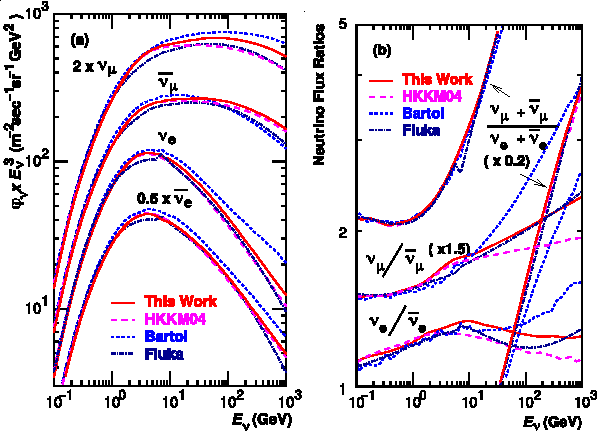
\includegraphics[width=0.7\textwidth]{pics/honda_flux.pdf}
	\captionof{figure}[Prediction of atmospheric neutrinos]%
	{Prediction of atmospheric neutrinos created with a 3D simulation %
	of Earth's atmosphere and including geomagnetic effects.
	Taken from~\cite{Honda:2004yz}.}
	\label{fig:honda_flux}
\end{figure}

The neutrinos are produced isotropically around the atmosphere with energies up to a few hundreds of TeV, %
peaking at tens of GeV, even though the energy distribution is flavour dependent.
Although the production point of neutrinos varies in altitude, with a most probable value around 15\,km,
for an experiment on the Earth's surface neutrinos are coming from all directions with the flight path depending %
on the zenith angle to the origin.
This means that the distance travelled by atmospheric neutrinos varies from a minimum of a few kilometres %
to a maximum equal to the Earth's diameter, \np{1.2e4}\,km.
It was observed by the Super-Kamiokande experiment that the ratio of flavours of neutrinos from %
positive and negative zenith angle were different, implying the presence of neutrino oscillation~\cite{Fukuda:1998mi}.
A correct prediction of the atmospheric flux becomes instrumental in studying oscillation physics; %
computational-intensive 3D simulations have reached state-of-the-art precision with negligible statistical errors %
thanks to the implementation of geomagnetic models~\cite{Honda:2004yz, Honda:2006qj}.

\subsection{Accelerator neutrinos}
\label{sec:nu_acc}

Atmospheric neutrinos provide an invaluable source for studying the properties of neutrinos, %
such as the squared mass differences and the mixing angles.
However, the uncertainty on the path lengths of neutrinos from production to detection can downgrade %
the precision of the measurement.
Accelerator facilities try to overcome this limitation.
Neutrino beams are derived from a similar mechanism that generates atmospheric neutrinos.
A proton beam directed on a fixed target typically yields a large number of pions and kaons, %
and also heavier mesons the amount of which depends on the energy of the protons and the choice of the target.
All these secondary particles decay leptonically or semi-leptonically via CC weak interactions thus creating a neutrino beam.
Pions and kaons principally decay into $\nu_\mu$ because two-body electronic modes are disfavoured %
by helicity suppression.
Muons decay in turn into equal numbers of $\nu_e$ and $\cj{\nu}_\mu$.
Other production sources of $\nu_e$ are the three-body decays of $K^0$ and $K^+$.
As an example, the parentage composition of the Booster Neutrino Beam flux~\cite{AguilarArevalo:2008yp} %
is shown in \reffig{fig:bnb_flux}, highlighting that pions are the main source of low energy neutrinos %
and kaons of energetic ones.
Above the neutral kaon mass, the first significant source of neutrino is given by the $D_s$ meson, %
for which helicity suppression again favours the production of heavy charged-leptons, %
and so $\tau$~leptons and $\nu_\tau$ are more likely to be emitted than the other flavours.
Each of the subsequent $\tau^+$ decays produces a $\cj{\nu}_\tau$.
The production of $D_s$ mesons however requires a very high energy proton beam and therefore %
for practical reasons this contribution is disregarded in most experiments.

\begin{figure}[t]
	\begin{minipage}[t]{0.48\textwidth}
		\centering
		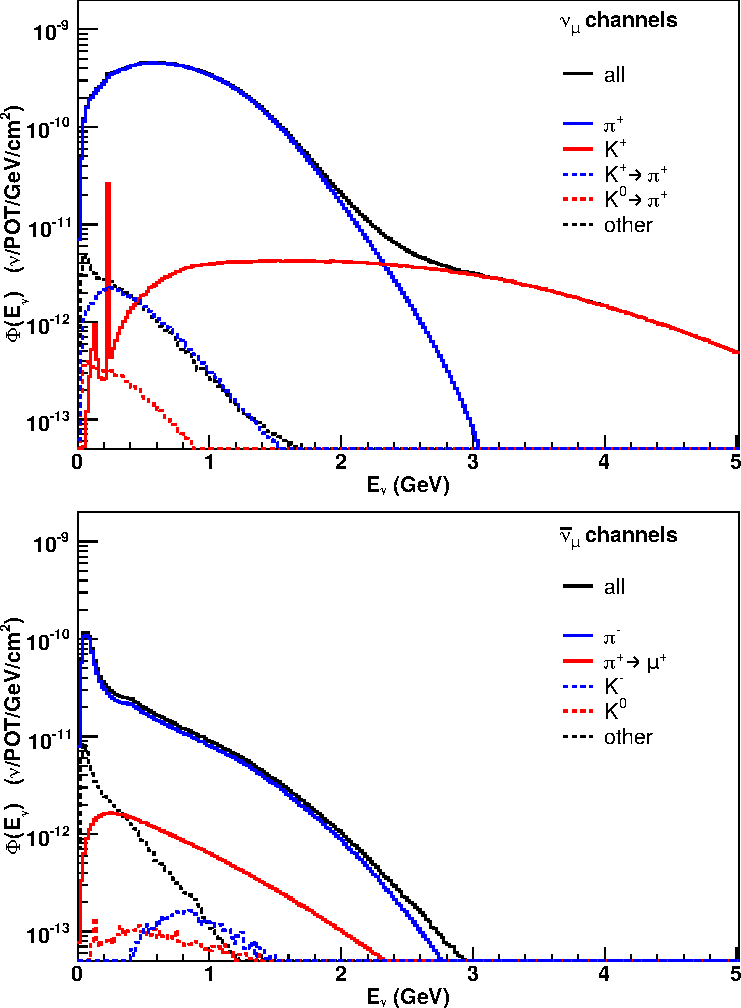
\includegraphics[width=\textwidth]{pics/bnb_flux.pdf}
		\captionof{figure}[Prediction of $\nu_\mu$ and $\cj{\nu}_\mu$ at the Booster Neutrino Beam]%
		{Prediction of the $\nu_\mu$ (top) and $\cj{\nu}_\mu$ (bottom) fluxes at the %
		Booster Neutrino Beam.
		The contributions from different parent particles are highlighted.
		Taken from \refref{AguilarArevalo:2008yp}.}
		\label{fig:bnb_flux}
	\end{minipage}
	\hfill
	\begin{minipage}[t]{0.48\textwidth}
		\centering
		\raisebox{3.0em}{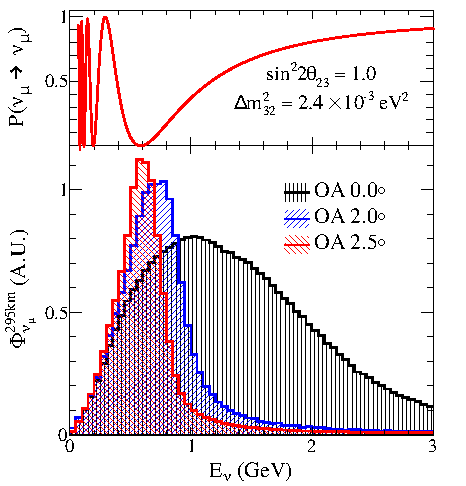
\includegraphics[width=\textwidth]{pics/t2k_flux.pdf}}
		\captionof{figure}[Prediction of $\nu_\mu$ at T2K]%
		{Prediction of the $\nu_\mu$ flux at T2K (bottom), %
		showing the profile at different off-axis angles (OA).
		At $2.5^\circ$ from the axis, the energy distributions peaks %
		in correspondence of a minimum for the $\nu_\mu$ disappearance probability (top).
	       	Taken from \refref{Abe:2012av}.}
		\label{fig:t2k_flux}
	\end{minipage}
\end{figure}



The energy and angular distributions of the neutrinos reflect the kinematic properties of %
the parent particles, which are in turn produced with a variety of angles and energies.
Given its wide angular distribution, the neutrino beam may not give rise to the high statistics %
required by typical long baseline oscillation experiments.
To improve the quality of the beam, a focusing system is typically put into place %
by partially surrounding the target with one or more pulsed toroidal electromagnets, called \emph{horns}.
The horns are activated with pulsed currents of hundreds of kilo-Ampere for a few microseconds %
in coincidence with the proton beam arriving at the target.
Within the horn cavity, the pulse creates a magnetic field that decreases %
radially with respect to the axis of the horn, meaning that the peak intensity of the magnetic field %
is reached at the inner regions of the toroid.
By changing the direction of the current in the horns it is possible to select and focus particles of the desired charge.
The configuration for which positively charged pions are focused and negatively ones are rejected is %
referred to as Forward Horn Current (FHC) and the resulting beam is mainly composed of neutrinos.
With a Reverse Horn Current (RHC) configuration, negative pions are selected and the beam is principally made of anti-neutrinos.
The two operation modes are also known as $\nu$-mode and $\cj{\nu}$-mode.
Despite the optimal design of the horn, kaons and short-lived mesons cannot be deflected as efficiently %
as pions and muons, and therefore the neutrino beam presents an intrinsic spread.
In certain cases, the neutrino experiment is located off the axis of the beam, as for the T2K~\cite{Abe:2012av} %
and NO$\nu$A~\cite{Ayres:2004js} experiments.
%Neutrinos emitted away from the beam-axis have an energy, At angles $\theta > 0$ the energy of the neutrino becomes independent of the %
%energy of the parent meson and
The energy distribution of neutrinos emitted away from the beam axis loses some dependancy from the parent meson %
and the profile becomes approximately monochromatic~\cite{Beavis_Carroll_Chiang_1995}.
This characteristic is favourable in oscillation experiment, in which the ratio between baseline and %
neutrino energy should be fixed and known, as shown in \reffig{fig:t2k_flux}.


\section{Neutrino interactions}
\label{sec:neutrino_interactions}

\begin{figure}
	\centering
	\medskip
	\begin{fmffile}{neutrino_CC}
		\begin{fmfgraph*}(80,60)
			\fmfleft{f1,nu}
			\fmfright{f2,ell}
			\fmf{fermion}{nu,v1,ell}
			\fmf{fermion}{f1,v2,f2}
			\fmf{photon, label=$W$}{v1,v2}
			\fmflabel{$\ferm_1$}{f1}
			\fmflabel{$\ferm_2$}{f2}
			\fmflabel{$\nu_\alpha$}{nu}
			\fmflabel{$\ell_\alpha$}{ell}
		\end{fmfgraph*}
	\end{fmffile}
	\qquad
	\raisebox{2.5em}{,}
	\qquad
	\begin{fmffile}{neutrino_NC}
		\begin{fmfgraph*}(80,60)
			\fmfleft{f1,nu1}
			\fmfright{f2,nu2}
			\fmf{fermion}{nu1,v1,nu2}
			\fmf{fermion}{f1,v2,f2}
			\fmf{photon, label=$Z$}{v1,v2}
			\fmflabel{$\ferm$}{f1}
			\fmflabel{$\ferm$}{f2}
			\fmflabel{$\nu_\alpha$}{nu1}
			\fmflabel{$\nu_\alpha$}{nu2}
		\end{fmfgraph*}
	\end{fmffile}
	\bigskip
	\caption[Generic CC and NC tree-level weak interactions]%
	{Generic CC (right) and NC (left) tree-level interactions with neutrinos involved.
	Note that these diagrams have illustration purpose only, and time flow convention is not respected. }
	\label{fig:neutrino_tree}
\end{figure}

Neutrino interactions in their flavour states are described by \refeqs{eq:lepton_cc}{eq:lepton_nc}.
Replacing the values of $g^\nu_V$ and $g^\nu_A$ for a neutrino, the relevant Lagrangian terms are
\begin{align}
	%\label{eq:real_lepton_cc}
	\mathcal{L}_{\text{CC},\nu} &= -\frac{g}{2\sqrt{2}}\ 	      %
	\sum_{\alpha=e,\mu,\tau} \cj{\nu}_\alpha \sh{W} (1-\gamma^5) \ell_\alpha + \text{h.c.}\ , \\
	%\label{eq:real_lepton_nc}
	\mathcal{L}_{\text{NC},\nu} &= -\frac{g}{4\cos\vartheta_\text{W}}\ %
	\sum_{\alpha=e,\mu,\tau} \cj{\nu}_\alpha \sh{Z} (1-\gamma^5) \nu_\alpha \ .
\end{align}
For energies below the $W$ and $Z$ mass, the allowed tree-level interactions involving at least one neutrino %
are any allowed variation of the processes represented in \reffig{fig:neutrino_tree}.
The vector bosons cannot be produced on-shell and so their field operator must contract with some other external field.
The amplitudes of the processes shown in \reffig{fig:neutrino_tree} are
\begin{align}
	i \mathcal{M}_\text{CC} &= i\, \frac{g^2}{8}\ \cj{u}_{\ell_\alpha} \gamma^\mu (1-\gamma^5)\, u_{\nu_\alpha}
						    \,\frac{\eta_{\mu\nu}}{k^2 - m_W^2+i\varepsilon}
						    \,\cj{u}_{\ferm_2} \gamma^\nu (1-\gamma^5)\,V_{12}\, u_{\ferm_1}\ , \\
	i \mathcal{M}_\text{NC} &= i\, \frac{g^2}{8\cos\vartheta}\ \cj{u}_{\nu_\alpha} \gamma^\mu (1-\gamma^5)\, u_{\nu_\alpha}
						    \,\frac{\eta_{\mu\nu}}{k^2 - m_Z^2+i\varepsilon}
						    \,\cj{u}_{\ferm} \gamma^\nu (g^\ferm_V-g^\ferm_A\gamma^5) u_{\ferm}\ ,
\end{align}
where $k$ is the momentum of the propagator and $V_{12}$ a possible mixing between generic fermions $\ferm_1$ and $\ferm_2$.
Because of the typical energies involved, the momentum propagating between the particles is small %
compared to the masses of the intermediate bosons and therefore their mass can be factorised out, %
resulting in the four-point interactions
\begin{align}
	\label{eq:fermi_cc}
	i \mathcal{M}_\text{CC} &\simeq i\,  \frac{G_F^2}{\sqrt{2}}\ \cj{u}_{\ell_\alpha} \gamma^\mu (1-\gamma^5)\, u_{\nu_\alpha}
						    \,\cj{u}_{\ferm_2} \gamma^\mu (1-\gamma^5)\,V_{12}\, u_{\ferm_1}\ , \\
	\label{eq:fermi_nc}
	i \mathcal{M}_\text{NC} &\simeq i\,  \frac{G_F^2}{\sqrt{2}}\ \cj{u}_{\nu_\alpha} \gamma^\mu (1-\gamma^5)\, u_{\nu_\alpha}
						    \,\cj{u}_{\ferm} \gamma^\mu (g^\ferm_V-g^\ferm_A\gamma^5) u_{\ferm}\ ,
\end{align}
where the relation in \refeq{eq:magic_ratio} was used and a new constant was introduced 
\begin{equation}
	\label{eq:fermi_const}
	\frac{G_F}{\sqrt{2}} = \frac{g^2}{8\,m_W^2}\ .
\end{equation}
The constant in \refeq{eq:fermi_const} is called Fermi's constant and the interactions %
can be described by effective four-point Lagrangian.
%\begin{align}
%	\mathcal{L}_\text{eff, CC} &= - \frac{G_F}{\sqrt{2}} \qty[\cj{\ell}_\alpha \gamma^\mu(1-\gamma^5)\nu_\alpha] %
%							     \qty[\cj{f}_2\gamma_\mu(1 - \gamma^5) f_1] \\
%	\mathcal{L}_\text{eff, CC} &= - \frac{G_F}{\sqrt{2}} \qty[\cj{\nu}_\alpha \gamma^\mu(1-\gamma^5)\nu_\alpha] %
%							     \qty[\cj{f}\gamma_\mu(g^F_V - g^F_A \gamma^5) f]
%\end{align}
						    
In the following sections the most important neutrino interactions with matter are reviewed, %
from low to high energies.

\subsection{Coherent elastic neutrino--nucleus scattering}
\label{sec:cevns}

The coupling of neutrinos to the $Z$ boson opens the possibility of a coherent interactions %
with all the nucleons in an atomic nucleus, if the momentum exchange  $q^2$ %
is significantly small~\cite{Freedman:1973yd}.
This interaction is called coherent elastic neutrino--nucleus scattering, or ``CE$\nu$NS''.
The coherence condition corresponds to target nucleons in phase with each other with $q^2 \lesssim 1/R^2$, %
where $R$ is the size of the nucleus.
This restricts the process to energies below a few tens of MeV.
However, the probability of interaction scales with the square nuclear mass, %
enhancing at low energies the cross-section with respect to the interaction with individual nucleons.
This is depicted in \reffig{fig:cevns}.
The signature of this reaction is a recoil of the target nucleus, since low-energy neutrinos are not easily detected.
The differential cross-section with respect to the recoil energy $T$ reads~\cite{Freedman:1973yd, Drukier:1983gj}
\begin{equation}
	%\dv{\sigma}{T} = \frac{G_F^2}{2\pi} M \qty[2 - \frac{2T}{E} + \qty(\frac{T}{E})^2 - \frac{MT}{E^2}] %
	%		\frac{Q_W^2}{4} F^2(q^2)\ .
	\dv{\sigma}{T} = \frac{G_F^2}{2\pi} M \qty[(G_V + G_A)^2 + (G_V-G_A)^2 \qty(1 - \frac{T}{E})^2 - %
				(G_V^2-G_A^2) \frac{M\,T}{E^2}]\ , %
\end{equation}
where $M$ is the mass of the target, $E$ the energy of the incoming neutrino and
\begin{align}
	G_V &= \qty[g_V^p\, Z + g_V^n\, N]\, F_V(q^2) \\
	G_A &= \qty[g_A^p\, (Z_+ - Z_-) + g_A^n\,(N_+ - N_-)]\, F_A(q^2)\ .
\end{align}
\begin{figure}
	\centering
	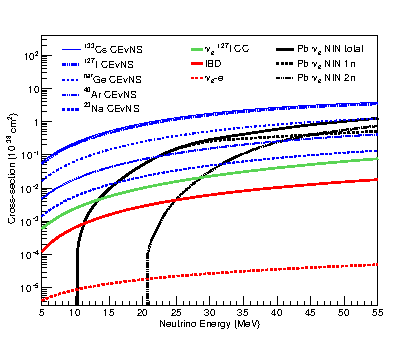
\includegraphics[width=0.7\textwidth]{pics/cevns.pdf}
	\caption[Neutrino--nucleus cross-sections at low neutrino energies]%
	{Behaviour of the neutrino--nucleus cross-sections for various targets, as a function of the neutrino energy.
	The cross-sections for neutrino-induced neutrons (NIN), inverse beta decay (IBD), and %
	elastic scattering of $\nu_e$ on electrons are also shown for comparison. Taken from~\refref{Akimov:2017ade}.}
	\label{fig:cevns}
\end{figure}
The vector and axial coupling constants for protons and neutrons are
\begingroup
\renewcommand*{\arraystretch}{1.25}
\begin{equation}
	\begin{array}{ll}
		g_V^p = \displaystyle\frac{1}{2} - 2 \sin^2\vartheta_\text{W} \ , & g_A^p =\displaystyle \frac{1}{2}\ , \\
		g_V^n = \displaystyle-\frac{1}{2} \ , & g_A^n = \displaystyle-\frac{1}{2} \ .\\
	\end{array}
\end{equation}
\endgroup
$Z_\pm$ and $N_\pm$ are respectively the number of protons and neutrons with spin up or spin down, %
and $F_V(q^2)$ and $F_A(q^2)$ are the vector and axial nuclear form factors.
The vector contribution dominates strongly for most nuclei, whereas the axial term %
shows an effect only on unpaired nucleons, which are typically just a few %
compared to the total number of nucleons or none for spin-zero nuclei.
Neglecting the axial form factor, at small recoils $T \lesssim E$ the cross-section simplifies to
\begin{equation}
	\dv{\sigma}{T} \simeq \frac{G_F^2}{8\pi} M F^2(q^2) \qty[N + (4\sin^2\vartheta_\text{W} - 1)Z]^2 %
				\qty(2 - \frac{MT}{E^2})\ .
\end{equation}
The angular dependence of the scattering is 
\begin{equation}
	\dv{\sigma}{\cos\theta} \simeq \frac{G_F^2}{8\pi} \qty[N + (4\sin^2\vartheta_\text{W} - 1)Z]^2 E (1 + \cos\theta)\ .
\end{equation}
Since $\sin^2\vartheta_\text{W} = 0.213$, the CE$\nu$NS cross-section is strongly dependent on the squared number of neutrons $N$, %
with a little contribution from the squared atomic number $Z$.



For heavy nuclei and sufficiently intense neutrino sources, %
the measurement of CE$\nu$NS can be achieved using relatively small active volumes.
This was first demonstrated by the COHERENT collaboration~\cite{Akimov:2015nza} which successfully %
observed the coherent scattering for the first time~\cite{Akimov:2017ade} using a \np{14.57}\,kg %
CsI[Na] scintillating crystal and collecting \np{1.76e23} protons on target.
The measurement of CE$\nu$NS is of utter importance for direct dark matter experiments, since the %
so-called \emph{neutrino floor} is due to CE$\nu$NS interactions of solar and atmospheric neutrinos.
This scattering also presents a chance for significant tests of the SM or searches of new physics, like non-standard neutrino %
interactions and the dark sector~\cite{Coloma:2017ncl} (see also \refref{Giunti:2019xpr}).



\subsection{Neutrino--electron scattering}
\label{sec:elastic_scattering}

The easiest interaction to study between neutrinos and matter components at low energies %
is the neutrino--electron elastic scattering
\begin{equation}
	\overset{(-)}{\nu}_\alpha + e^- \rightarrow \overset{(-)}{\nu}_\alpha + e^-\ .
\end{equation}
%The respective Feynman diagrams are shown in Fig.~\ref{fig:nescat} and~\ref{nutscat}.
%The effective lagrangian 
%\begin{align}
%	\mathcal{L}_\mathrm{eff}(\nu_e e^- \rightarrow \nu_e e^-) &= - \frac{G_F}{\sqrt{2}} %
%	[\overline{\nu_e}\gamma^\mu(1-\gamma^5)\nu_e][\bar{e}\gamma_\mu((1+g_V^l)-(1+g_A^l)\gamma^5)e] \\
%	\mathcal{L}_\mathrm{eff}(\nu_\alpha e^- \rightarrow \nu_\alpha e^-) &= - \frac{G_F}{\sqrt{2}} %
%	[\overline{\nu_\alpha}\gamma^\mu(1-\gamma^5)\nu_\alpha][\bar{e}\gamma_\mu(g_V^l-g_A^l)\gamma^5)e] %
%	\quad (\alpha = \mu,\tau)\,.
%\end{align}
Using the effective four-point Lagrangians, one can calculate the differential cross-sections in the laboratory frame %
with an initial electron at rest:
\begin{equation}
	\label{eq:nu_elastic_xsec}
	\dv{\sigma}{q^2} = \frac{G_F^2}{\pi} \qty[\kappa_1^2 + \kappa_2^2 
		\qty(1 - \frac{q^2}{2\,(p_\nu \cdot p_e)} )^2 - \kappa_1\, \kappa_2\, m_e^2\, \frac{q^2}{2\, (p_\nu \cdot p_e)^2} ] \ ,
\end{equation}
where the quantities $\kappa_1$ and $\kappa_2$ %
depend on the neutrino flavour and embeds CC and NC contributions.
Using the vector and axial coupling of \refeq{eq:gv_ga} they read
\begin{align}
	&\kappa_1^{\nu_e} = \kappa_2^{\cj{\nu}_e} = 1 + \frac{g_V^\ell + g_A^\ell}{2} = \frac{1}{2} + \sin^2\vartheta_\text{W}\ , \\
	&\kappa_2^{\nu_e} = \kappa_1^{\cj{\nu}_e} = \frac{g_V^\ell - g_A^\ell}{2} = \sin^2\vartheta_\text{W}\ , \\
	&\kappa_1^{\nu_{\mu,\tau}} = \kappa_2^{\cj{\nu}_{\mu,\tau}} = \frac{g_V^\ell + g_A^\ell}{2} = -\frac{1}{2} + \sin^2\vartheta_\text{W}\ , \\
	&\kappa_2^{\nu_{\mu,\tau}} = \kappa_1^{\cj{\nu}_{\mu,\tau}} = \frac{g_V^\ell - g_A^\ell}{2} = \sin^2\vartheta_\text{W} \ .
\end{align}
The quantity $q^2$ is the squared difference between the four-momentum of the initial and final electrons, 
and denoting $T_e = E_e - m_e$ as the kinetic energy of the outgoing electron, it follows
\begin{equation}
	q^2 = 2\,m_e\,T_e\ .
\end{equation}
With some kinematics, the kinetic energy is found to be
\begin{equation}
	T_e = \frac{2\,m_e\,E_\nu^2 \cos^2 \theta}{(m_e + E_\nu)^2 - E_\nu^2 \cos^2\theta}\ ,
\end{equation}
and so the differential cross-section in \refeq{eq:nu_elastic_xsec} can be given as a function of the %
electron scattering angle $\theta$ with respect to the incoming neutrino with energy $E_\nu$:
\begin{align}
	\dv{\sigma}{\cos\theta} =&\ \frac{2 G_F^2 m_e}{\pi} %
			\frac{4 E_\nu^2 (m_e+E_\nu)^2 \cos \theta}{\qty[(m_e+E_\nu)^2-E_\nu^2 \cos^2 \theta ]^2} \quad \times \notag \\
			&\qty[g_1^2 + g_2^2\qty(1 - \frac{2 m_e E_\nu \cos^2 \theta}{(m_e+E_\nu)^2-E_\nu^2 \cos^2 \theta} )^2 \!\!
		- \frac{2m_e^2 \cos^2 \theta\  g_1\, g_2}{(m_e+E_\nu)^2-E_\nu^2 \cos^2 \theta}]\ .
\end{align}

For the electron neutrino $\nu_e$, both CC and NC interactions are allowed and %
for the electron antineutrino $\cj{\nu}_e$ the $s$-channel and $t$-channel diagrams are swapped,
whereas for $\alpha = \mu, \tau$ only neutral-current interactions exist.
It results that the total cross-section for $\cj{\nu}_e$, $\nu_{\mu,\tau}$, and $\cj{\nu}_{\mu,\tau}$ %
are approximately and respectively 42\,\%, 16\,\%, and 14\,\% of the total cross-section of electron neutrinos, %
which goes for $\sqrt{s} \gg m_e$~as 
\begin{equation}
	\sigma_{\nu_e} \simeq \np{93e-46}\,\text{cm}^2\,\frac{s}{\text{MeV}}\ .
\end{equation}
The proportions between these interaction probabilities has been an important discriminant %
in solving the solar neutrino problem (see \refsec{sec:nu_sun_sn}).


\subsection{Neutrino scattering with nucleons}
\label{sec:ccqe}

At higher energies, the dominant neutrino interaction mode is with nucleons in matter, %
thanks to the $W$ and $Z$ couplings of the quark components and the currents of \refeqs{eq:real_quark_cc}{eq:real_quark_nc}.
In general, these processes can be categorised according to the momentum transfer.
At small $q^2$, elastic interactions dominate and may be brought about by both charged and neutral currents.
When this occurs via neutral currents, all flavour of neutrinos and anti-neutrinos can scatter off %
both neutrons and protons in what is referred to as ``NC elastic'' (NCE) scattering.
The process is the same for neutrinos and antineutrinos:
\begin{equation}
	\nu_\alpha + N \rightarrow \nu_\alpha + N \quad \text{or} \quad \bar\nu_\alpha + N \rightarrow \bar\nu_\alpha + N\ .
\end{equation}
Once neutrinos acquire sufficient energy they can also undergo the analogous charged current interactions, %
called ``quasi-elastic'' (CCQE), due to the fact that the recoiling nucleon changes its charge and mass transfer occurs.
The processes are
\begin{equation}
	\nu_\alpha + n \to p + \ell_\alpha^- \quad \text{and} \quad \bar\nu_\alpha + p \to n + \ell_\alpha^+ \ ,
\end{equation}
with $\alpha =e, \mu, \tau$.
The process for $\cj{\nu}_e$ is referred to as \emph{inverse beta decay} (IBD) and it is the principal mode %
of detection of electron anti-neutrinos~\cite{Vogel:1999zy}.
The differential cross-sections for the CCQE scattering in the laboratory frame are given by
\begin{align}
	\label{eq:cc_xsec_q}
	\frac{\mathrm{d} \sigma_{CC}}{\mathrm{d}q^2} &= \frac{G_F^2\,|V_{ud}|^2\,m_N^4}{8\pi\,(p_\nu \cdot p_N)^2} %
	\qty[A(q^2) \pm B(q^2) \frac{s-u}{m_N^2} + C(q^2) \frac{(s-u)^2}{m_N^4}]\ , \\
	\label{eq:cc_xsec_t}
	\frac{\mathrm{d} \sigma_{CC}}{\mathrm{d}\cos\theta} &= -\frac{G_F^2 |V_{ud}|^2 m_N^2}{4\pi} \frac{p_l}{E_\nu} %
	\qty[A(q^2) \pm B(q^2) \frac{s-u}{m_N^2} + C(q^2) \frac{(s-u)^2}{m_N^4}]\ ,
\end{align}
where $N$ denotes the nucleon and the plus sign refers to $N = n$ and the minus sign to $N = p$.
The functions $A(q^2)$, $B(q^2)$, and $C(q^2)$ for the charged-current process are:
\begin{align}
	A(q^2) &= \frac{m_l^2+q^2}{m_N^2} \bigg\{ \qty(1+\frac{q^2}{4m_N^2}) G_A^2 - \qty(1-\frac{q^2}{4m_N^2}) %
			\qty(F_1^2 - \frac{q^2}{4m_N^2}F_2^2 ) +\frac{q^2}{m_N^2}\,F_1\,F_2\notag \\
	\label{eq:A_Q}
		&\hphantom{=\frac{m_l^2+q^2}{m_N^2}}%\{}
			- \frac{m_l^2}{4m_N^2} %
		 \qty[ (F_1+F_2)^2+(G_A+2G_P)^2-\frac{1}{4}\qty(1+\frac{q^2}{4m_N^2}) G_P^2] \bigg\}\ ,\\
	\label{eq:B_Q}
	B(q^2) &= \frac{q^2}{m_N^2}\, G_A\, (F_1+F_2)\ ,\\
	\label{eq:C_Q}
	C(q^2) &= \frac{1}{4} \qty(G_A^2 +F_1^2+\frac{q^2}{4m_N^2}\,F_2^2)\ .
\end{align}
The terms $F_1$, $F_2$, $G_A$, and $G_P$ are form factors and are functions of $q^2$.
The nucleon form factors $F_1 = F_1^p - F_1^n$, $F_2 = F_2^p - F_2^n$ are known respectively as %
\emph{Dirac} and \emph{Pauli} form factors.
For $q^2 = 0$, they simplify to
\begingroup
\renewcommand*{\arraystretch}{1.25}
\begin{equation}
	\begin{array}{ll}
		F_1^p (0) = 1 \ , & F_1^n(0) = 0\ , \\
		F_2^p (0) = \displaystyle \frac{2\,m_p\,\mu_p}{e \hbar} - 1 \ , & F_2^n = \displaystyle \frac{2\,m_p\,\mu_n}{e\hbar} \ ,\\
	\end{array}
\end{equation}
\endgroup
where $\mu_p$ and $\mu_n$ are the proton and neutron magnetic momenta. %
For $q^2 \neq 0$ they are more conveniently described by the Sachs electric and magnetic momenta~\cite{Ernst:1960zza}.
The \emph{pseudo-scalar} form factor $G_P$ is usually ignored in cross-section calculations, %
whereas the \emph{axial} form factor is parameterised as
\begin{equation}
	\label{eq:axial_mass}
	G_A(q^2) = \frac{g_A}{\qty(1 + \displaystyle \frac{q^2}{m_A^2})^2}\ .
\end{equation}
All the form factors are usually fitted from data of neutrino experiments, %
since they give non-negligible contributions to the systematic uncertainties, %
particularly the \emph{axial mass} $m_A$ which is assumed to be $m_A = 1.0$\,GeV in many %
neutrino event generators.
%$G_A(q^2)$, and $G_P(q^2)$ 
The NCQE cross-sections have the same form as the ones in \refeqs{eq:cc_xsec_q}{eq:cc_xsec_t}, %
apart from the mixing term $|V_{ud}|^2$ and the corresponding neutral-current form factors
\begin{equation}
	F^N_{1,2} = \pm \frac{1}{2} (F_{1,2}^p - F_{1,2}^n) - %
			2 \sin^2 \vartheta_\text{W} F_{1,2}^N - \frac{1}{2} F_{1,2}^N\ ,
\end{equation}
where the plus sign is for $N = p$ and the minus sign for $N = n$.

CCQE interactions are of vital importance for neutrino physics, because %
the measurement of its differential cross-section give precious information on the nucleon form-factors, %
which are difficult to measure with a different probe.
Also, the two-body nature of the interactions is such that the kinematic properties of the %
incoming neutrino can be determined with good precision.
This is relevant especially for oscillation experiments, in which the energy of the neutrino %
can be estimated from the momentum of the outgoing charge lepton $p_\ell$ and its angle %
with the direction of the incoming neutrino $\theta_\ell$, if known.
If the target nucleon is at rest compared to the neutrino energy, %
then this can be calculated as:
\begin{equation}
	\label{eq:e_reco}
	E_\nu = \frac{m_n E_\ell + \frac{1}{2}\big ( m_p^2-m_n^2-m_\ell^2)}{m_n - E_\ell+p_\ell \cos \theta_\ell}\ .
\end{equation}

\begin{figure}
	\centering
	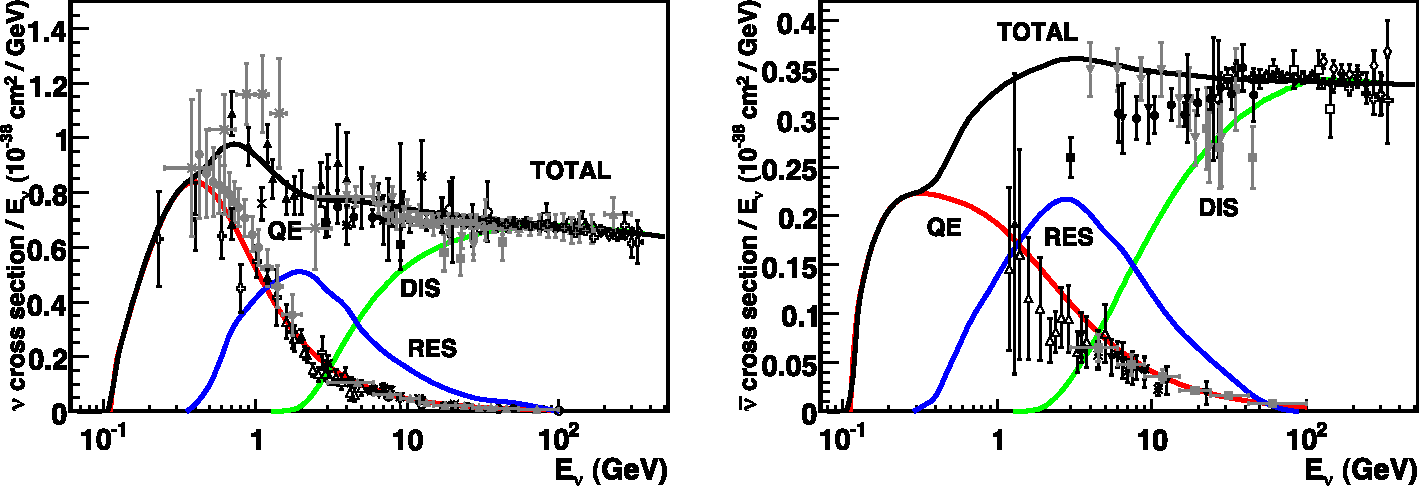
\includegraphics[width=\textwidth]{pics/qe_xsec.pdf}
	\caption[Neutrino--nucleus cross-sections at high neutrino energies]%
	{Total neutrino (left) and antineutrino (right) cross-section measurements and predictions for an isoscalar target %
	as a function of energy. The contributions from quasi-elastic (QE, red), resonance (RES, blue), %
	and deep-inelastic-scattering (DIS, green) are highlighted.
	Resonant modes only give a substantial contribution in a small energy region between 1\,GeV and 7\,GeV, %
	explaining the difficulty in constraining theoretical models.
	Taken from~\refref{Formaggio:2013kya}.}
	\label{fig:xsec}
\end{figure}

The neutrino--hadron cross-sections as a functions of energy are shown in \reffig{fig:xsec}.
The QE cross-section drops for neutrino energies above 1\,GeV as the available $q^2$ increases. 
At higher energies, processes such as multi-nucleon emission or baryon resonance become relevant.
%In this kind of interactions,
Correlated pairs of nucleons inside the nucleus can be simultaneously ejected, in the so-called $2p2h$ interactions, %
or the nucleon itself gets excited into a baryonic resonance before decaying and emitting a charged or a neutral pion.
There are many theoretical models explaining these multi-body interactions~\cite{Rein:1980wg, Martini:2009uj, Nieves:2011pp}, %
and neutrino interaction generators, like GENIE~\cite{Andreopoulos:2009rq} or NEUT~\cite{Hayato:2002sd}, %
often implement more than one.
The determination of the correct paradigm is a hard task, due to the difficulty of the measurement of resonant modes.
In fact, at high $q^2$ or for $E_\nu \gtrsim 8$\,GeV deep inelastic scattering (DIS) is the dominant mode, since %
the neutrino has enough energy to scatter directly off a constituent quark and to fragment the original nucleon.
